%%%%%%%%%%%%%%%%%%%%%%%%%%%%%%%%%%%%%%%%%
% Focus Beamer Presentation
% LaTeX Template
% Version 1.0 (8/8/18)
%
% This template has been downloaded from:
% http://www.LaTeXTemplates.com
%
% Original author:
% Pasquale Africa (https://github.com/elauksap/focus-beamertheme) with modifications by 
% Vel (vel@LaTeXTemplates.com)
%
% Template license:
% GNU GPL v3.0 License
%
% Important note:
% The bibliography/references need to be compiled with bibtex.
%
%%%%%%%%%%%%%%%%%%%%%%%%%%%%%%%%%%%%%%%%%

%----------------------------------------------------------------------------------------
%	PACKAGES AND OTHER DOCUMENT CONFIGURATIONS
%----------------------------------------------------------------------------------------
\documentclass{beamer}
\usepackage{lmodern}						
\usepackage[T1]{fontenc}		
\usepackage[utf8]{inputenc}	
\usepackage{lipsum}
\usepackage{lastpage}			
\usepackage{indentfirst}		
\usepackage{color}			
\usepackage{graphicx}			
\usepackage{microtype} 			
\usepackage{amsmath}
\usepackage{psfrag}
\usepackage{amsfonts}
\usepackage{amssymb}
\usepackage{tabularx}
\usepackage{lscape}
\usepackage{rotating}
\usepackage{multirow}
\usepackage{tikz}
\usepackage{physics}
\usepackage{pgfplots}
\usepackage{pgfplotstable}
\usetikzlibrary{matrix,chains,arrows,shapes.multipart,automata,calc,fit,tikzmark,trees,shapes}

\usetheme{focus} % Use the Focus theme supplied with the template
% Add option [numbering=none] to disable the footer progress bar
% Add option [numbering=fullbar] to show the footer progress bar as always full with a slide count

% Uncomment to enable the ice-blue theme
%\definecolor{main}{RGB}{92, 138, 168}
%\definecolor{background}{RGB}{240, 247, 255}https://www.overleaf.com/project/5ee63eecb6cd7b00012c03e1

%------------------------------------------------
%\usepackage{pgfplots}

\usepackage{booktabs} % Required for better table rules

%----------------------------------------------------------------------------------------
%	 TITLE SLIDE
%----------------------------------------------------------------------------------------

\title{Compara\c{c}\~ao de t\'ecnicas de \\aprendizagem de m\'aquina e\\ processamento de sinal para BCIs}

%\subtitle{Subtitle}

\author{Aluno: Otto Luiz A. Glass \\ Orientador: Thiago da Silva Castro}

\titlegraphic{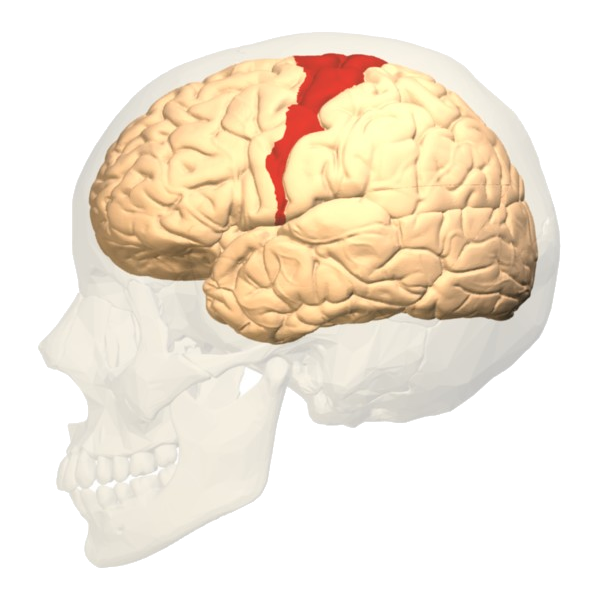
\includegraphics[scale=0.15]{Images/brain.png}} % Optional title page image, comment this line to remove it

\institute{Instituto Federal Sudeste MG \\ Campus Juiz de Fora}

\date{14 06 2020}

%------------------------------------------------

\begin{document}

%------------------------------------------------

\begin{frame}
	\maketitle % Automatically created using the information in the commands above
\end{frame}

%----------------------------------------------------------------------------------------
%	 SECTION 1
%----------------------------------------------------------------------------------------

%\section{Introdu\c{c}\~ao}
\begin{frame}{Etapas da Interface}
    \begin{columns}
        \begin{column}{0.5\textwidth}
           \begin{center}
               \begin{figure}
                   \centering
                   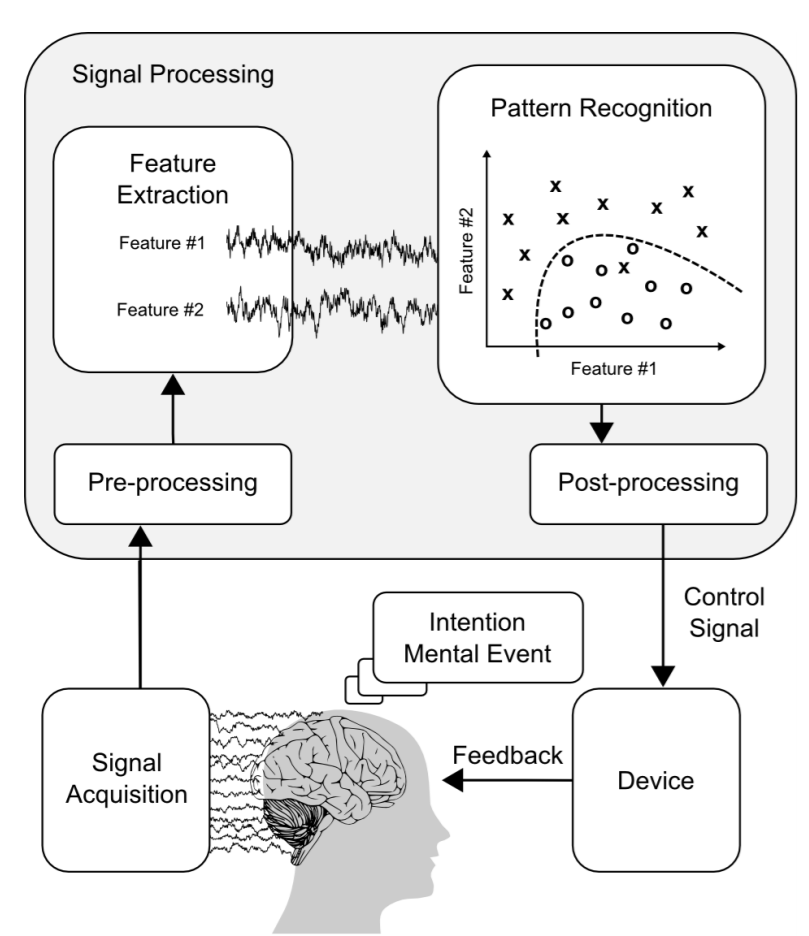
\includegraphics[scale=.30]{Images/bci-stages.png}
                   \caption{Etapas BCI\cite{Rao2010}}
                   \label{fig:Estagio_BCI}
               \end{figure}
           \end{center}
       \end{column}
       \begin{column}{0.5\textwidth}
       \begin{itemize}
           \item Sinal: Ondas $\mu$
           \item Extra\c{c}\~ao de caracteristicas: STFT, Espectro de Welch e Multitaper
           \item Reconhecimento de pad\~oes: Redes Neurais, SVM e Vizinhos Proximos
       \end{itemize}
       \end{column}
    \end{columns}
\end{frame}
%------------------------------------------------

\begin{frame}{Ritimo $\mu$}
    \begin{columns}
        \begin{column}{0.5\textwidth}
           \begin{center}
               \begin{figure}
                   \centering
                   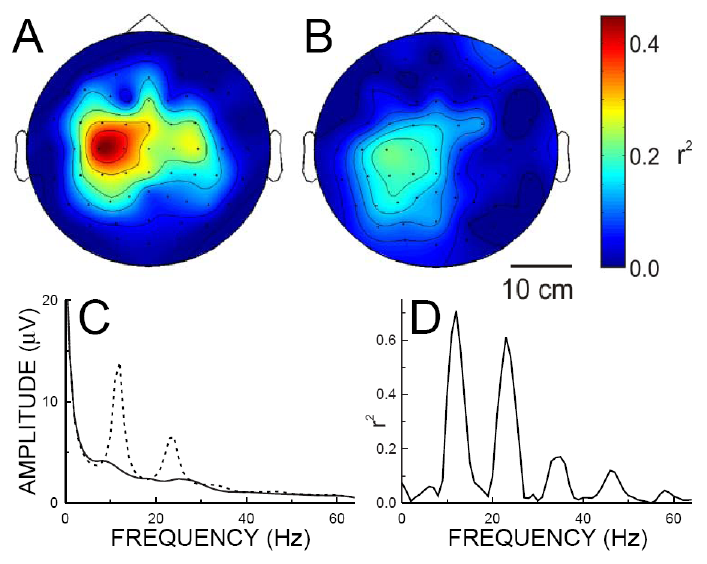
\includegraphics[scale=0.25]{Images/ERDmu.PNG}
                   \caption{\cite{BCI2000}}
                   \label{fig:Estagio_BCI}
               \end{figure}
           \end{center}
         \end{column}
         \begin{column}{0.5\textwidth}
            \begin{itemize}
                \item Componente principal $10Hz$ Amplitude $10\mu$ - $20\mu$
                \item Presente na aus\^encia de movimento
            \end{itemize}
         \end{column}
    \end{columns}               
\end{frame}
%------------------------------------------------

\begin{frame}{Ritimo $\mu$}
    \begin{columns}
        \begin{column}{0.5\textwidth}
           \begin{center}
               \begin{figure}
                   \centering
                   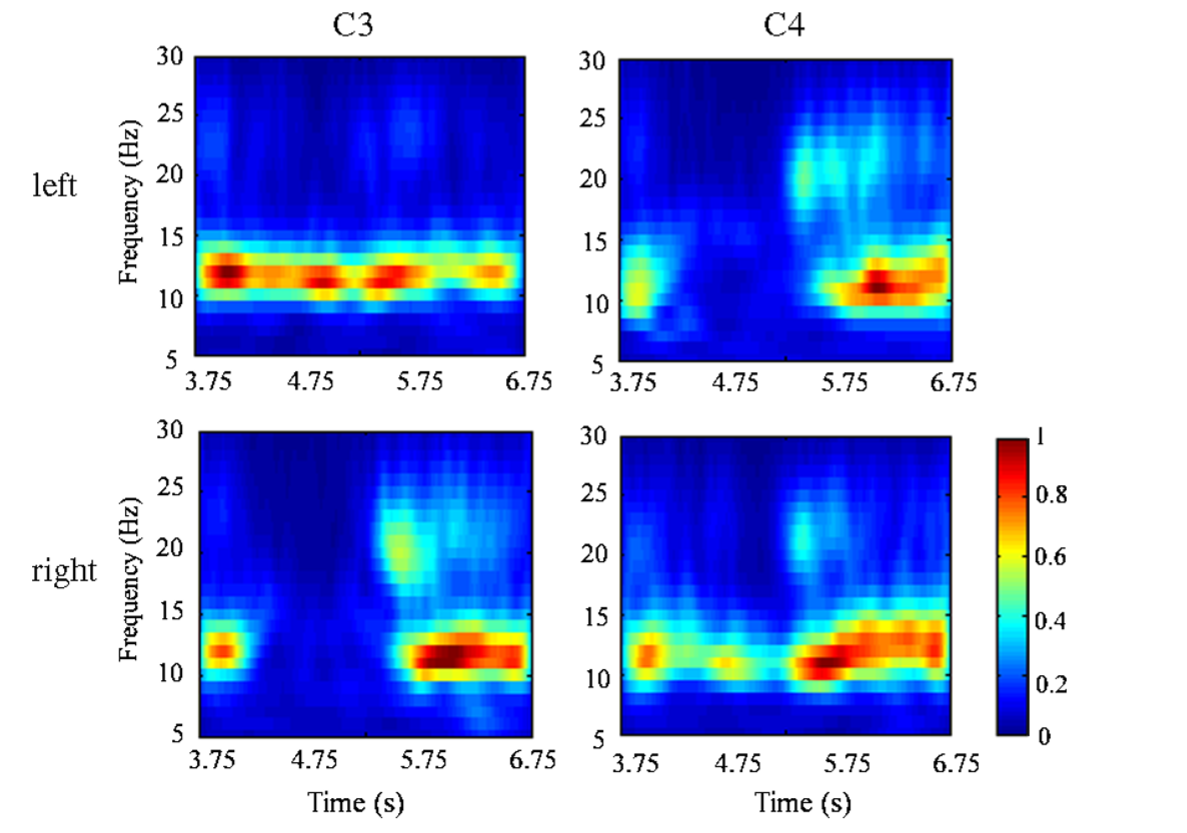
\includegraphics[scale=0.25]{Images/mu-left-vs-right.png}
                   \caption{\cite{Qin2004}}
                   \label{fig:Estagio_BCI}
               \end{figure}
           \end{center}
         \end{column}
         \begin{column}{0.5\textwidth}
            \begin{figure}
                \centering
               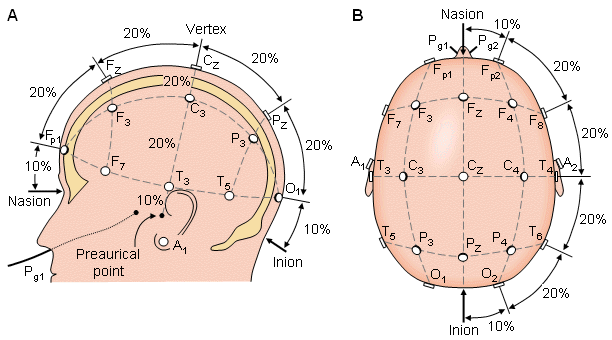
\includegraphics[scale=0.45]{Images/10-20_cranio.png}
               \caption{\cite{EEGPrinciple}}
               \label{fig:Estagio_BCI}
            \end{figure}
         \end{column}
    \end{columns}           
\end{frame}

%------------------------------------------------
%---------------Filtragem EOG--------------------
%------------------------------------------------
\begin{frame}{Filtragem EOG}
    \begin{columns}
        \begin{column}{0.5\textwidth}
           \begin{center}
               \begin{figure}
                   \centering
                   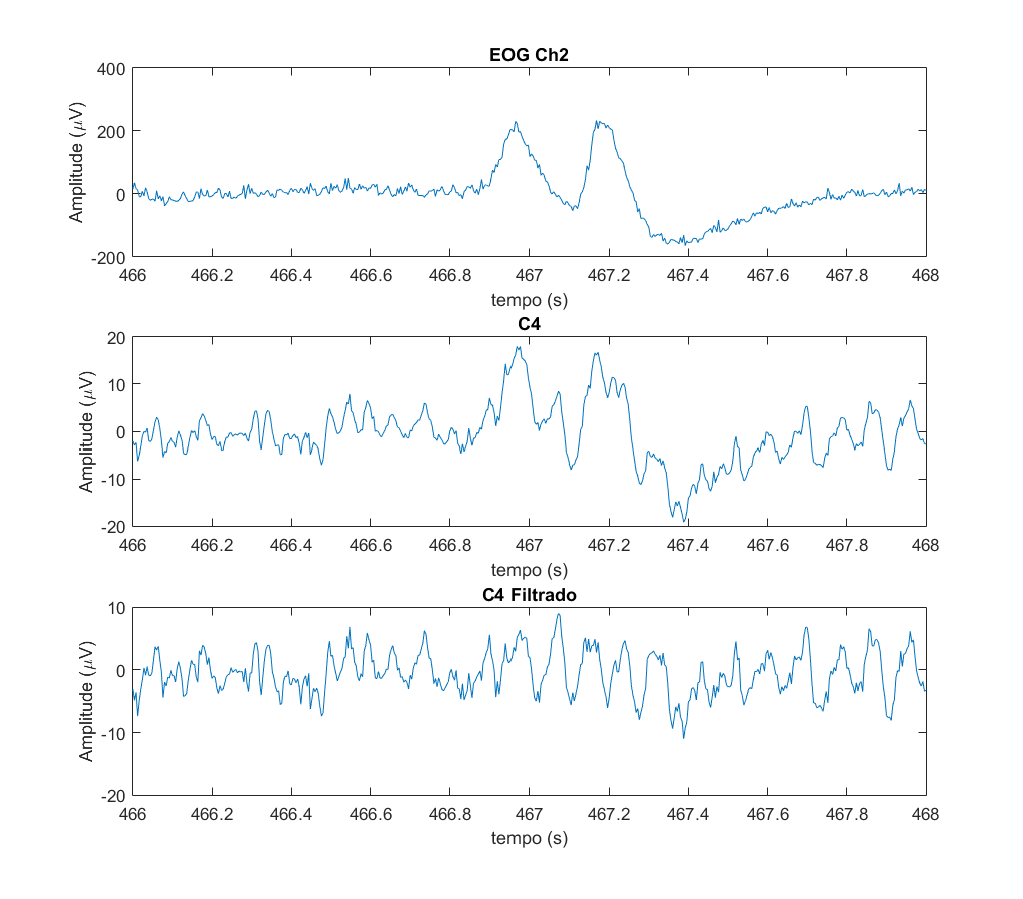
\includegraphics[scale=0.20]{Images/FiltragemEOG.png}
                  % \caption{\cite{Qin2004}}
                  % \label{fig:Fil}
               \end{figure}
           \end{center}
         \end{column}
        % \begin{column}{0.5\textwidth}
         %   \begin{itemize}
         %       \item
        %    \end{itemize}
        % \end{column}
    \end{columns}           
\end{frame}


%\section{Metodologia} % Section title slide, unnumbered

%------------------------------------------------

\begin{frame}{Dataset}

 	\centering
 	\begin{table}[]
        \begin{tabular}{lll}
        \hline
        ID & Training               & Evalutation    \\ \hline
        1  & B0101T, B0102T, B0103T & B0101E, B0102E \\
        2  & B0201T, B0202T, B0203T & B0201E, B0202E \\
        3  & B0301T, B0302T, B0303T & B0301E, B0302E \\
        4  & B0401T, B0402T, B0403T & B0401E, B0402E \\
        5  & B0501T, B0502T, B0503T & B0501E, B0502E \\
        6  & B0601T, B0602T, B0603T & B0601E, B0602E \\
        7  & B0701T, B0702T, B0703T & B0701E, B0702E \\
        8  & B0801T, B0802T, B0803T & B0801E, B0802E \\
        9  & B0901T, B0902T, B0903T & B0901E, B0902E \\ \hline
        \end{tabular}
        \end{table}
 	 \caption{ \cite{GrazBData}}	
 	\label{fig:Data-Graz}
\end{frame}
%------------------------------------------------

\begin{frame}{Amostras}
 \begin{figure}[h!]
 	\centering
 	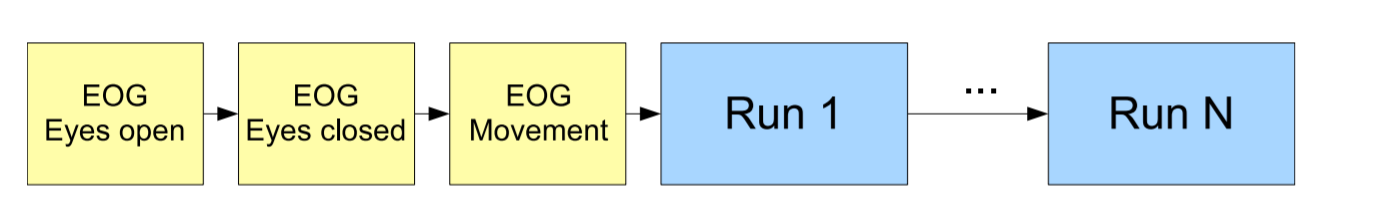
\includegraphics[scale=0.42]{./Images/graz-eog}
 	 \caption{Segmento EOG nas sess\~oes do graz-b \cite{GrazBData}}	
 	\label{fig:Graz-EOG}
 \end{figure}
\end{frame}
%------------------------------------------------

\begin{frame}{Sessões}
  \begin{figure}[h!]
  	\centering
 	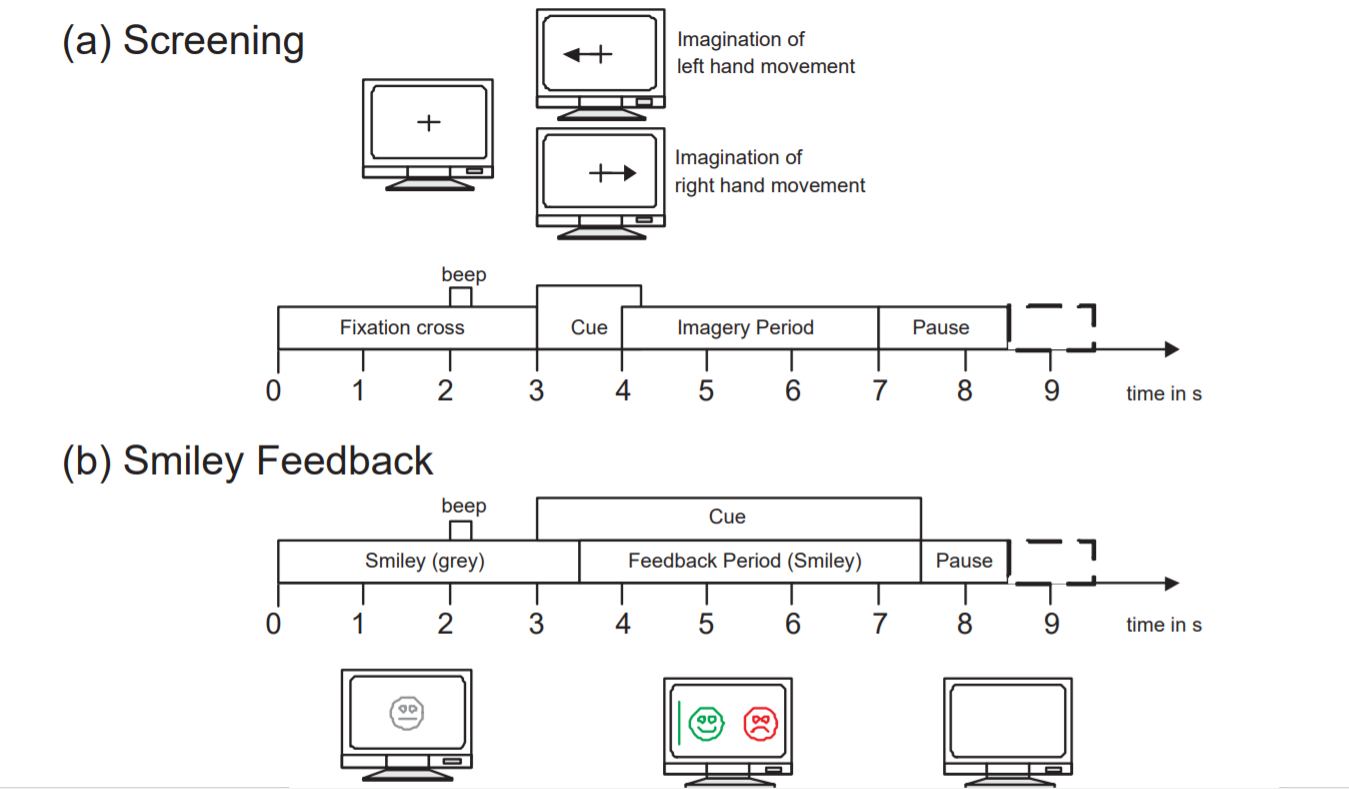
\includegraphics[scale=0.35]{./Images/graz_b_session}
 	 \caption{Os dois tipos de sess\~ao em Graz-b \cite{GrazBData}.}
 	\label{fig:Graz-Session}
 \end{figure}
\end{frame}
%--------------------------------------------------
   
%\section{Teoria}

%--------------------------------------------------
\begin{frame}{Sampling}
%\begin{center}
\color{black}
\scalebox{.7}{
	\tikzstyle{sample}=[minimum height=1cm,minimum width=4cm,xshift=2cm,draw=black]
\tikzstyle{plotsf}=[smooth,yscale=0.05,xscale=8,color=blue]
%\tikzstyle{lines}=[color=black,line width=0.5mm]
\tikzstyle{lines}=[color=black,very thick]
\begin{tikzpicture}[
 brc/.style args = {#1/#2}{decorate,
	decoration={brace, amplitude=5pt,
		raise=#1,#2},% for mirroring of brace
	thick},]
%\begin{axis}[axis line style={draw=none},
%tick style={draw=none},]
%	\addplot table[y=y,x=t,col sep=comma] {./dados/EEG2.csv};
%\end{axis}
\draw (0,0)  [plotsf] plot file {./dados/EEG2.table};
\draw [lines, dashdotted ](2cm,0.5cm)--(2cm,-4cm);
\draw [lines, dashdotted ](4cm,0.5cm)--(4cm,-4cm);
\draw [lines](2cm,-3.5cm)--(4cm,-3.5cm) node [midway,below] {\textbf{overlap}};
\draw [thick,double,->] (4.5cm,-3cm)--(4.5cm,-4cm)--(10cm,-4cm) node [midway,below]{\tiny{\textbf{Extra\c{c}\~ao de caracter\'isticas}}};
\draw (0,0) node (s0) [sample,minimum width=16cm,xshift=6cm]{};
\begin{scope}[yshift=-1.25cm]
\draw (0,0) [plotsf] plot file {./dados/EEG1-1.table};
\draw (0,0) node (s1) [sample] {};
\end{scope}
\node (s1text) [right=of s1,xshift=-1cm]{Janela 1};
\begin{scope}[yshift=-2.5cm]
\draw (0,0)[plotsf] plot  file {./dados/EEG1-2.table};
\draw (0,0) node (s2) [sample,xshift=2cm] {};
\end{scope}
\node (s1text) [right=of s2,xshift=-1cm]{Janela 2};
\begin{scope}[xshift=10cm,yshift=-5cm]
\begin{scope}[scale=0.6]
\begin{axis}[%axis line style={draw=none},
tick style={draw=none},
]
	\addplot table[y=P,x=f,col sep=comma] {./dados/EEGWelch2.csv};
\end{axis}
\end{scope}
\end{scope}
\draw[brc=2mm/](0,0.5)--(16,0.5) node [midway,above,yshift=6]{\textbf{Experimento}};
\end{tikzpicture}}
%\end{center}
\end{frame}
%--------------------------------------------------

\begin{frame}{Processamento de Sinais}
\scalebox{.8}{
\tikzstyle{sample}=[minimum height=1cm,minimum width=4cm,xshift=2cm,draw=black]
\tikzstyle{plotsf}=[smooth,yscale=0.05,xscale=8,color=blue]
%\tikzstyle{lines}=[color=black,line width=0.5mm]
\tikzstyle{lines}=[color=black,very thick]
\begin{tikzpicture}[
 brc/.style args = {#1/#2}{decorate,
	decoration={brace, amplitude=5pt,
		raise=#1,#2},% for mirroring of brace
	thick},]
%\begin{axis}[axis line style={draw=none},
%tick style={draw=none},]
%	\addplot table[y=y,x=t,col sep=comma] {./dados/EEG2.csv};
%\end{axis}
\begin{scope}[xshift=0cm,yshift=-2.5cm]
\draw (0,0)[plotsf] plot  file {./dados/EEG1-2.table};

\draw (0,0) node (s2) [sample,xshift=2cm] {};
\end{scope}

tick style={draw=none},
]
\draw [thick,double,color=black] (4.5cm,-3cm)--(4.5cm,-4cm)--(8cm,-4cm) node [below]{\tiny{\textbf{Extra\c{c}\~ao de caracter\'isticas}}} node [above]{$f(t)\rightarrow F(S)$};
\draw [thick,double,->,color=black] (8cm,-4cm)--(10cm,-4cm)--(10cm,-3cm) ;
\begin{scope}[xshift=8.5cm,yshift=-3cm,xscale=.02,yscale=-.15,rotate=-90]%,xcomb]
\draw (0,0) [color=black]rectangle (15,150);
\draw (0,0)[color=blue,thick]  plot  file {./dados/EEGWelch2.table};
\end{scope}
\end{tikzpicture}
}
\end{frame}
%--------------------------------------------------

\begin{frame}{Espectro de Welch}
            \color{black}

\scalebox{.6}{
\tikzstyle{sample}=[minimum height=1cm,minimum width=4cm,xshift=2cm,draw=black]
\tikzstyle{plotsf}=[smooth,yscale=0.05,xscale=8,color=blue]
%\tikzstyle{lines}=[color=black,line width=0.5mm]
\tikzstyle{lines}=[color=black,very thick]
\begin{tikzpicture}[
 brc/.style args = {#1/#2}{decorate,
	decoration={brace, amplitude=5pt,
		raise=#1,#2},% for mirroring of brace
	thick},]
%\begin{axis}[axis line style={draw=none},
%tick style={draw=none},]
%	\addplot table[y=y,x=t,col sep=comma] {./dados/EEG2.csv};
%\end{axis}
\draw (0,0)  [plotsf] plot file {./dados/EEG2.table};
%\draw [thick,double,->] (4.5cm,-3cm)--(4.5cm,-4cm)--(10cm,-4cm) node [midway,below]{\tiny{\textbf{Extra\c{c}\~ao de caracter\'isticas}}};
\draw (0,0) node (s0) [sample,minimum width=16cm,xshift=6cm]{};
\draw [lines, dashdotted ](5.5cm,0.5cm)--(5.5cm,-.5cm);
\draw [lines, dashdotted ](11cm,0.5cm)--(11cm,-0.5cm);
%---------------------------
%Setas para as Janelas FFT
\draw [-latex,very thick](3cm,-0.5cm)--(3cm,-1.8cm)  node[midway,left]{$\hat{S}_1(f)$};
\draw [-latex,very thick](8.5cm,-0.5cm)--(8.5cm,-1.8cm)  node[midway,left]{$\hat{S}_2(f)$};
\draw [-latex,very thick](14cm,-0.5cm)--(14cm,-1.8cm)  node[midway,left]{$\hat{S}_k(f)$};
%---------------------------
%Graficos FFT Janelas
%1
\begin{scope}[xshift=1cm,yshift=-5cm,xscale=-.03,yscale=-.014,rotate=180]%,xcomb]
\draw (-5,0) [color=black,thick]rectangle (125,230);
\draw (0,0)[color=blue,thick]  plot  file {./dados/Welch/W1.table};
\end{scope}
%2
\begin{scope}[xshift=6.5cm,yshift=-5cm,xscale=-.03,yscale=-.014,rotate=180]%,xcomb]
\draw (-5,0) [color=black,thick]rectangle (125,230);
\draw (0,0)[color=blue,thick]  plot  file {./dados/Welch/W2.table};
\end{scope}
%3
\begin{scope}[xshift=12cm,yshift=-5cm,xscale=-.03,yscale=-.014,rotate=180]%,xcomb]
\draw (-5,0) [color=black,thick]rectangle (125,230);
\draw (0,0)[color=blue,thick]  plot  file {./dados/Welch/W3.table};
\end{scope}
%---------------------------
%Espectro de Welch

\begin{scope}[xshift=6.5cm,yshift=-10.5cm,xscale=-.03,yscale=-.014,rotate=180]%,xcomb]
\draw (-5,0) [color=black,thick]rectangle (125,230);
\draw (0,0)[color=blue,thick]  plot  file {./dados/Welch/WMean.table};
\end{scope}
%---------------------------
%SUM
\begin{scope}[xshift=8.3cm,yshift=-6cm]
\node[circle,thick,draw=black] (0,0) {\huge{$+$}};
\end{scope}
%SUM ARROWS
\draw [-latex,very thick](3cm,-5cm)--(3cm,-6cm)--(7.9cm,-6cm);
\draw [-latex,very thick](8.3cm,-5cm)--(8.3cm,-5.5cm);
\draw [-latex,very thick](14cm,-5cm)--(14cm,-6cm)--(8.7cm,-6cm);
%MEAN ARROW
\draw [-latex,very thick](8.3cm,-6.35cm)--(8.3cm,-7.25cm) node[midway,left]{$\frac{1}{K}$};


\end{tikzpicture}
}
\end{frame}
%--------------------------------------------------

\begin{frame}{Multitaper}
            \color{black}

\scalebox{.5}{
\tikzstyle{sample}=[minimum height=1cm,minimum width=4cm,xshift=2cm,draw=black]
\tikzstyle{plotsf}=[smooth,yscale=0.05,xscale=8,color=blue,]
\tikzstyle{lines}=[color=black,very thick]
\begin{tikzpicture}[
 brc/.style args = {#1/#2}{decorate,
	decoration={brace, amplitude=5pt,
		raise=#1,#2},% for mirroring of brace
	thick},]
	

\begin{scope}[xscale=0.7,yscale=.3]
\begin{axis}[%axis line style={draw=none},
tick style={draw=blue}, yticklabels={,,}, xticklabels={,,},mark repeat=50,ticks=none
]
	\addplot[color=blue] table[y=EEG,x=t,col sep=comma] {./dados/Multitaper/multitaper_all.csv};
\end{axis}
\end{scope}
%----------------------------Tapered EEG--------------
%1
\begin{scope}[xscale=0.7,yscale=.3,yshift=7cm,xshift=8cm]
\begin{axis}[%axis line style={draw=none},
tick style={draw=blue}, yticklabels={,,}, xticklabels={,,},mark repeat=50,ticks=none
]
	\addplot[color=red,loosely dashdotted,very thick] table[y=S1,x=t,col sep=comma] {./dados/Multitaper/multitaper_all.csv};
	\addplot[color=blue] table[y=ES1,x=t,col sep=comma] {./dados/Multitaper/multitaper_all.csv};
\end{axis}
\end{scope}
%2
\begin{scope}[xscale=0.7,yscale=.3,xshift=8cm]
\begin{axis}[%axis line style={draw=none},
tick style={draw=blue}, yticklabels={,,}, xticklabels={,,},mark repeat=50,ticks=none
]
	\addplot[color=red,loosely dashdotted,very thick] table[y=S2,x=t,col sep=comma] {./dados/Multitaper/multitaper_all.csv};
	\addplot[color=blue] table[y=ES2,x=t,col sep=comma] {./dados/Multitaper/multitaper_all.csv};
\end{axis}
\end{scope}
%3
\begin{scope}[xscale=0.7,yscale=.3,yshift=-7cm,xshift=8cm]
\begin{axis}[%axis line style={draw=none},
tick style={draw=blue}, yticklabels={,,}, xticklabels={,,},mark repeat=50,ticks=none
]
	\addplot[color=red,loosely dashdotted,very thick] table[y=S3,x=t,col sep=comma] {./dados/Multitaper/multitaper_all.csv};
	\addplot[color=blue] table[y=ES3,x=t,col sep=comma] {./dados/Multitaper/multitaper_all.csv};
\end{axis}
\end{scope}
%---------------------------Tapered PSDs--------------------
%1
\begin{scope}[xscale=0.55,yscale=.3,yshift=7cm,xshift=21cm]
\begin{axis}[%axis line style={draw=none},
tick style={draw=blue}, yticklabels={,,}, xticklabels={,,},mark repeat=50,ticks=none
]
	\addplot[color=blue] table[y=TS1,x=f,col sep=comma] {./dados/Multitaper/multitaper_all.csv};
\end{axis}
\end{scope}
%2
\begin{scope}[xscale=0.55,yscale=.3,xshift=21cm]
\begin{axis}[%axis line style={draw=none},
tick style={draw=blue}, yticklabels={,,}, xticklabels={,,},mark repeat=50,ticks=none
]
	\addplot[color=blue] table[y=TS2,x=f,col sep=comma] {./dados/Multitaper/multitaper_all.csv};
\end{axis}
\end{scope}
%3
\begin{scope}[xscale=0.55,yscale=.3,yshift=-7cm,xshift=21cm]
\begin{axis}[%axis line style={draw=none},
tick style={draw=blue}, yticklabels={,,}, xticklabels={,,},mark repeat=50,ticks=none
]
	\addplot[color=blue] table[y=TS3,x=f,col sep=comma] {./dados/Multitaper/multitaper_all.csv};
\end{axis}
\end{scope}
%---------------------------------Multitaper---------
\begin{scope}[xscale=0.55,yscale=.3,xshift=32cm]
\begin{axis}[%axis line style={draw=none},
tick style={draw=blue}, yticklabels={,,}, xticklabels={,,},mark repeat=50,ticks=none
]
	\addplot[color=blue] table[y=PSD,x=f,col sep=comma] {./dados/Multitaper/multitaper_all.csv};
\end{axis}
\end{scope}
%-----------------Sum-------------------------
\begin{scope}[xshift=16.5cm,yshift=.8cm]
\node[circle,thick,draw=black] (0,0) {\huge{$+$}};
\end{scope}
%-----------------Arrows----------------------
%-------EEG To Tapered-------
%1
\draw [-latex,very thick](3cm,1.7cm)--(3cm,3cm)--(5.6cm,3cm) node[midway,above]{$\times T_1$};
%2
\draw [-latex,very thick](4.8cm,.8cm)--(5.6cm,.8cm) node[midway,above]{$\times T_2$};
%3
\draw [-latex,very thick](3cm,0cm)--(3cm,-1.4cm)--(5.6cm,-1.4cm) node[midway,above]{$\times T_k$};
%--------Tapered To PSDs------
%1
\draw [-latex,very thick](10.4cm,3cm)--(11.6cm,3cm) node[midway,above]{$\hat{S}_1(f)$};

%2
\draw [-latex,very thick](10.4cm,.8cm)--(11.6cm,.8cm) node[midway,above]{$\hat{S}_2(f)$};

%3
\draw [-latex,very thick](10.4cm,-1.4cm)--(11.6cm,-1.4cm) node[midway,above]{$\hat{S}_k(f)$};
%--------PSDS to Sum-----------
%1
\draw [-latex,very thick](15.3cm,3cm)--(16.5cm,3cm) --(16.5cm,1.2cm) ;

%2
\draw [-latex,very thick](15.3cm,.8cm)--(16.1cm,.8cm) ;

%3
\draw [-latex,very thick](15.3cm,-1.4cm)--(16.5cm,-1.4cm) --(16.5cm,.3cm) ;
%----------Average----------
\draw [-latex,very thick](16.9cm,.8cm)--(17.6cm,.8cm) node[midway,above]{$\frac{1}{K}$};
\end{tikzpicture}
}
\end{frame}

%--------------------------------------------------
\begin{frame}{Aprendizado de Maquinas}
\color{black}

%\scalebox{.4}{\tikzset{%
  every neuron/.style={
    circle,
    draw,
    minimum size=1cm
  },
  neuron missing/.style={
    draw=none, 
    scale=2,
    text height=0.333cm,
    execute at begin node=\color{black}$\vdots$
  },
  every input/.style={
  	rectangle,
  	draw,
  	minimum size=0.2cm
  },
  input missing/.style={
	draw=none, 
	scale=2,
	text height=0.333cm,
	execute at begin node=\color{black}$\vdots$
},
}

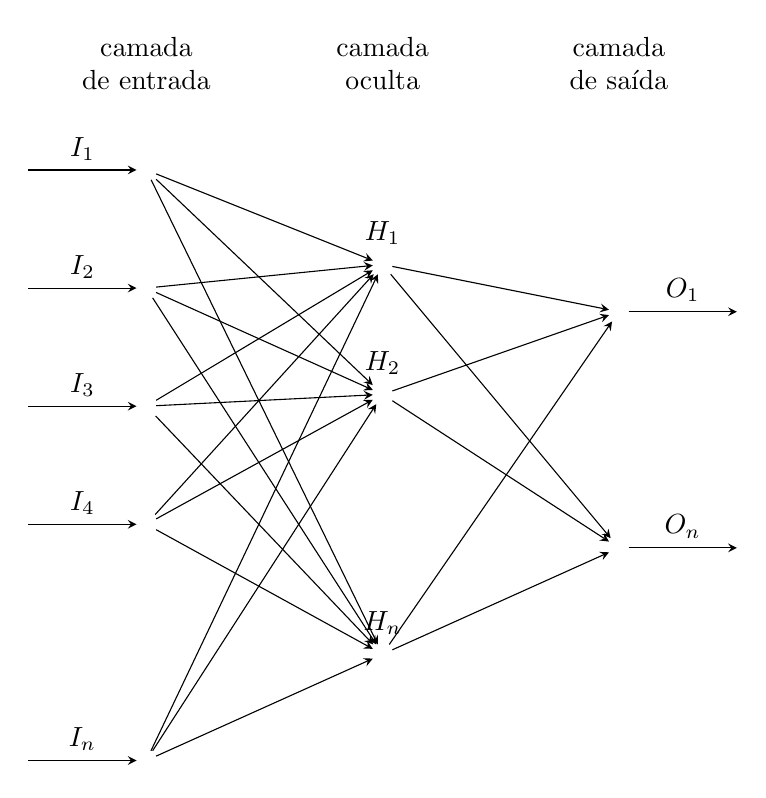
\begin{tikzpicture}[x=1.5cm, y=1.5cm, >=stealth]

\foreach \m/\l [count=\y] in {1,2,3,4,missing,5}
  \node [every input/.try, input \m/.try] (input-\m) at (0,2.7-\y) {};

\foreach \m [count=\y] in {1,2,missing,3}
  \node [every neuron/.try, neuron \m/.try ] (hidden-\m) at (2,2-\y*1.1) {};

\foreach \m [count=\y] in {1,missing,2}
  \node [every neuron/.try, neuron \m/.try ] (output-\m) at (4,1.5-\y) {};

\foreach \l [count=\i] in {1,2,3,4,n}
  \draw [<-] (input-\i) -- ++(-1,0)
    node [above, midway] {$I_\l$};

\foreach \l [count=\i] in {1,2,n}
  \node [above] at (hidden-\i.north) {$H_\l$};

\foreach \l [count=\i] in {1,n}
  \draw [->] (output-\i) -- ++(1,0)
    node [above, midway] {$O_\l$};

\foreach \i in {1,...,5}
  \foreach \j in {1,...,3}
    \draw [->] (input-\i) -- (hidden-\j);

\foreach \i in {1,...,3}
  \foreach \j in {1,...,2}
    \draw [->] (hidden-\i) -- (output-\j);

\foreach \l [count=\x from 0] in {de entrada, oculta, de sa\'ida}
  \node [align=center, above] at (\x*2,2.3) {camada \\ \l};

\end{tikzpicture}}
%\scalebox{.5}{%\begin{tikzpicture}[&gt;=stealth']
\begin{tikzpicture}
% Draw axes
%\draw [&lt;-&gt;,thick] (0,5) node (yaxis) [above] {$y$}
\draw [thick] (0,5) node (yaxis) [above] {$y$}
|- (5,0) node (xaxis) [right] {$x$};
% draw line
\draw (0,-1) -- (5,4); % y=x-1
\draw[dashed] (-1,0) -- (4,5); % y=x+1
\draw[dashed] (2,-1) -- (6,3); % y=x-3
\draw[black,<->,very thick]     (1.5,2.5)-- (3.5,0.5) node[above, rotate=-45,midway,xshift=-5]{$D$};% y=-x+4
% \draw labels
\draw (3.5,3) node[rotate=45,font=\small] 
{$\mathbf{w}\cdot \mathbf{x} + b = 0$};
\draw (2.5,4) node[rotate=45,font=\small] 
{$\mathbf{w}\cdot \mathbf{x} + b = 1$};
\draw (4.5,2) node[rotate=45,font=\small] 
{$\mathbf{w}\cdot \mathbf{x} + b = -1$};
% draw distance
%\draw[dotted] (4,5) -- (6,3);
%\draw (5.25,4.25) node[rotate=-45] {$\frac{2}{\Vert \mathbf{w} \Vert}$};
%\draw[dotted] (0,0) -- (0.5,-0.5);
%\draw (0,-0.5) node[rotate=-45] {$\frac{b}{\Vert \mathbf{w} \Vert}$};
%\draw[-&gt;] (2,1) -- (1.5,1.5);
%\draw[thick] (2,1) -- (1.5,1.5);
\draw (1.85,1.35) node[rotate=-45]{}; %{$\mathbf{w}$};
% draw negative dots
\fill[red] (0.5,1.5) circle (3pt);
\fill[red]   (2.5,3.5)   circle (3pt);
\fill[black] (1,2.5)     circle (3pt);
\fill[black] (0.75,2)    circle (3pt);
\fill[black] (0.6,1.9)   circle (3pt);
\fill[black] (0.77, 2.5) circle (3pt);
\fill[black] (1.5,3)     circle (3pt);
\fill[black] (1.3,3.3)   circle (3pt);
\fill[black] (0.6,3.2)   circle (3pt);
% draw positive dots
\draw[red,thick] (4,1)     circle (3pt); 
\draw[red,thick] (3.3,.3)  circle (3pt); 
\draw[black]     (4.5,1.2) circle (3pt); 
\draw[black]     (4.5,.5)  circle (3pt); 
\draw[black]     (3.9,.7)  circle (3pt); 
\draw[black]     (5,1)     circle (3pt); 
\draw[black]     (3.5,.2)  circle (3pt); 
\draw[black]     (4,.3)    circle (3pt); 
\end{tikzpicture}}
\vspace{1cm}
\scalebox{.6}{
\tikzset{%
  every neuron/.style={
    circle,
    draw,
    minimum size=1cm
  },
  neuron missing/.style={
    draw=none, 
    scale=2,
    text height=0.333cm,
    execute at begin node=\color{black}$\vdots$
  },
  every input/.style={
  	rectangle,
  	draw,
  	minimum size=0.2cm
  },
  input missing/.style={
	draw=none, 
	scale=2,
	text height=0.333cm,
	execute at begin node=\color{black}$\vdots$
},
}

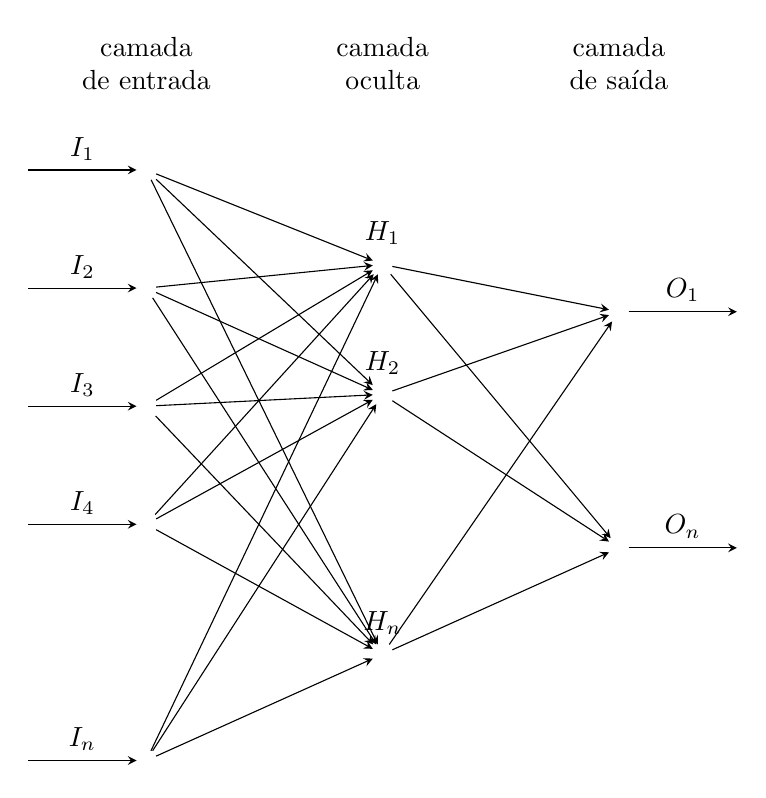
\begin{tikzpicture}[x=1.5cm, y=1.5cm, >=stealth]

\foreach \m/\l [count=\y] in {1,2,3,4,missing,5}
  \node [every input/.try, input \m/.try] (input-\m) at (0,2.7-\y) {};

\foreach \m [count=\y] in {1,2,missing,3}
  \node [every neuron/.try, neuron \m/.try ] (hidden-\m) at (2,2-\y*1.1) {};

\foreach \m [count=\y] in {1,missing,2}
  \node [every neuron/.try, neuron \m/.try ] (output-\m) at (4,1.5-\y) {};

\foreach \l [count=\i] in {1,2,3,4,n}
  \draw [<-] (input-\i) -- ++(-1,0)
    node [above, midway] {$I_\l$};

\foreach \l [count=\i] in {1,2,n}
  \node [above] at (hidden-\i.north) {$H_\l$};

\foreach \l [count=\i] in {1,n}
  \draw [->] (output-\i) -- ++(1,0)
    node [above, midway] {$O_\l$};

\foreach \i in {1,...,5}
  \foreach \j in {1,...,3}
    \draw [->] (input-\i) -- (hidden-\j);

\foreach \i in {1,...,3}
  \foreach \j in {1,...,2}
    \draw [->] (hidden-\i) -- (output-\j);

\foreach \l [count=\x from 0] in {de entrada, oculta, de sa\'ida}
  \node [align=center, above] at (\x*2,2.3) {camada \\ \l};

\end{tikzpicture}
%\begin{tikzpicture}[&gt;=stealth']
\begin{tikzpicture}
% Draw axes
%\draw [&lt;-&gt;,thick] (0,5) node (yaxis) [above] {$y$}
\draw [thick] (0,5) node (yaxis) [above] {$y$}
|- (5,0) node (xaxis) [right] {$x$};
% draw line
\draw (0,-1) -- (5,4); % y=x-1
\draw[dashed] (-1,0) -- (4,5); % y=x+1
\draw[dashed] (2,-1) -- (6,3); % y=x-3
\draw[black,<->,very thick]     (1.5,2.5)-- (3.5,0.5) node[above, rotate=-45,midway,xshift=-5]{$D$};% y=-x+4
% \draw labels
\draw (3.5,3) node[rotate=45,font=\small] 
{$\mathbf{w}\cdot \mathbf{x} + b = 0$};
\draw (2.5,4) node[rotate=45,font=\small] 
{$\mathbf{w}\cdot \mathbf{x} + b = 1$};
\draw (4.5,2) node[rotate=45,font=\small] 
{$\mathbf{w}\cdot \mathbf{x} + b = -1$};
% draw distance
%\draw[dotted] (4,5) -- (6,3);
%\draw (5.25,4.25) node[rotate=-45] {$\frac{2}{\Vert \mathbf{w} \Vert}$};
%\draw[dotted] (0,0) -- (0.5,-0.5);
%\draw (0,-0.5) node[rotate=-45] {$\frac{b}{\Vert \mathbf{w} \Vert}$};
%\draw[-&gt;] (2,1) -- (1.5,1.5);
%\draw[thick] (2,1) -- (1.5,1.5);
\draw (1.85,1.35) node[rotate=-45]{}; %{$\mathbf{w}$};
% draw negative dots
\fill[red] (0.5,1.5) circle (3pt);
\fill[red]   (2.5,3.5)   circle (3pt);
\fill[black] (1,2.5)     circle (3pt);
\fill[black] (0.75,2)    circle (3pt);
\fill[black] (0.6,1.9)   circle (3pt);
\fill[black] (0.77, 2.5) circle (3pt);
\fill[black] (1.5,3)     circle (3pt);
\fill[black] (1.3,3.3)   circle (3pt);
\fill[black] (0.6,3.2)   circle (3pt);
% draw positive dots
\draw[red,thick] (4,1)     circle (3pt); 
\draw[red,thick] (3.3,.3)  circle (3pt); 
\draw[black]     (4.5,1.2) circle (3pt); 
\draw[black]     (4.5,.5)  circle (3pt); 
\draw[black]     (3.9,.7)  circle (3pt); 
\draw[black]     (5,1)     circle (3pt); 
\draw[black]     (3.5,.2)  circle (3pt); 
\draw[black]     (4,.3)    circle (3pt); 
\end{tikzpicture}}
%\input{./graficos/KNN2.tex}

\end{frame}
%--------------------------------------------------

\begin{frame}{Redes Neurais}
    \begin{columns}
        \begin{column}{0.5\textwidth}            
            \color{black}
            
            %\scalebox{.4}{\tikzset{%
  every neuron/.style={
    circle,
    draw,
    minimum size=1cm
  },
  neuron missing/.style={
    draw=none, 
    scale=2,
    text height=0.333cm,
    execute at begin node=\color{black}$\vdots$
  },
  every input/.style={
  	rectangle,
  	draw,
  	minimum size=0.2cm
  },
  input missing/.style={
	draw=none, 
	scale=2,
	text height=0.333cm,
	execute at begin node=\color{black}$\vdots$
},
}

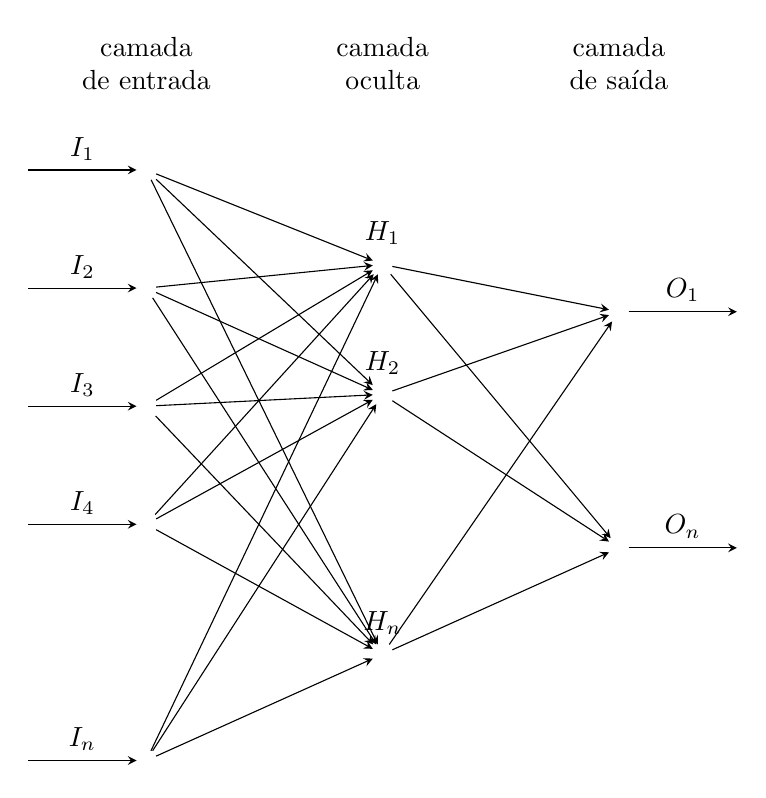
\begin{tikzpicture}[x=1.5cm, y=1.5cm, >=stealth]

\foreach \m/\l [count=\y] in {1,2,3,4,missing,5}
  \node [every input/.try, input \m/.try] (input-\m) at (0,2.7-\y) {};

\foreach \m [count=\y] in {1,2,missing,3}
  \node [every neuron/.try, neuron \m/.try ] (hidden-\m) at (2,2-\y*1.1) {};

\foreach \m [count=\y] in {1,missing,2}
  \node [every neuron/.try, neuron \m/.try ] (output-\m) at (4,1.5-\y) {};

\foreach \l [count=\i] in {1,2,3,4,n}
  \draw [<-] (input-\i) -- ++(-1,0)
    node [above, midway] {$I_\l$};

\foreach \l [count=\i] in {1,2,n}
  \node [above] at (hidden-\i.north) {$H_\l$};

\foreach \l [count=\i] in {1,n}
  \draw [->] (output-\i) -- ++(1,0)
    node [above, midway] {$O_\l$};

\foreach \i in {1,...,5}
  \foreach \j in {1,...,3}
    \draw [->] (input-\i) -- (hidden-\j);

\foreach \i in {1,...,3}
  \foreach \j in {1,...,2}
    \draw [->] (hidden-\i) -- (output-\j);

\foreach \l [count=\x from 0] in {de entrada, oculta, de sa\'ida}
  \node [align=center, above] at (\x*2,2.3) {camada \\ \l};

\end{tikzpicture}}
            %\scalebox{.5}{%\begin{tikzpicture}[&gt;=stealth']
\begin{tikzpicture}
% Draw axes
%\draw [&lt;-&gt;,thick] (0,5) node (yaxis) [above] {$y$}
\draw [thick] (0,5) node (yaxis) [above] {$y$}
|- (5,0) node (xaxis) [right] {$x$};
% draw line
\draw (0,-1) -- (5,4); % y=x-1
\draw[dashed] (-1,0) -- (4,5); % y=x+1
\draw[dashed] (2,-1) -- (6,3); % y=x-3
\draw[black,<->,very thick]     (1.5,2.5)-- (3.5,0.5) node[above, rotate=-45,midway,xshift=-5]{$D$};% y=-x+4
% \draw labels
\draw (3.5,3) node[rotate=45,font=\small] 
{$\mathbf{w}\cdot \mathbf{x} + b = 0$};
\draw (2.5,4) node[rotate=45,font=\small] 
{$\mathbf{w}\cdot \mathbf{x} + b = 1$};
\draw (4.5,2) node[rotate=45,font=\small] 
{$\mathbf{w}\cdot \mathbf{x} + b = -1$};
% draw distance
%\draw[dotted] (4,5) -- (6,3);
%\draw (5.25,4.25) node[rotate=-45] {$\frac{2}{\Vert \mathbf{w} \Vert}$};
%\draw[dotted] (0,0) -- (0.5,-0.5);
%\draw (0,-0.5) node[rotate=-45] {$\frac{b}{\Vert \mathbf{w} \Vert}$};
%\draw[-&gt;] (2,1) -- (1.5,1.5);
%\draw[thick] (2,1) -- (1.5,1.5);
\draw (1.85,1.35) node[rotate=-45]{}; %{$\mathbf{w}$};
% draw negative dots
\fill[red] (0.5,1.5) circle (3pt);
\fill[red]   (2.5,3.5)   circle (3pt);
\fill[black] (1,2.5)     circle (3pt);
\fill[black] (0.75,2)    circle (3pt);
\fill[black] (0.6,1.9)   circle (3pt);
\fill[black] (0.77, 2.5) circle (3pt);
\fill[black] (1.5,3)     circle (3pt);
\fill[black] (1.3,3.3)   circle (3pt);
\fill[black] (0.6,3.2)   circle (3pt);
% draw positive dots
\draw[red,thick] (4,1)     circle (3pt); 
\draw[red,thick] (3.3,.3)  circle (3pt); 
\draw[black]     (4.5,1.2) circle (3pt); 
\draw[black]     (4.5,.5)  circle (3pt); 
\draw[black]     (3.9,.7)  circle (3pt); 
\draw[black]     (5,1)     circle (3pt); 
\draw[black]     (3.5,.2)  circle (3pt); 
\draw[black]     (4,.3)    circle (3pt); 
\end{tikzpicture}}
            \vspace{1cm}
            \scalebox{.6}{
            \tikzset{%
  every neuron/.style={
    circle,
    draw,
    minimum size=1cm
  },
  neuron missing/.style={
    draw=none, 
    scale=2,
    text height=0.333cm,
    execute at begin node=\color{black}$\vdots$
  },
  every input/.style={
  	rectangle,
  	draw,
  	minimum size=0.2cm
  },
  input missing/.style={
	draw=none, 
	scale=2,
	text height=0.333cm,
	execute at begin node=\color{black}$\vdots$
},
}

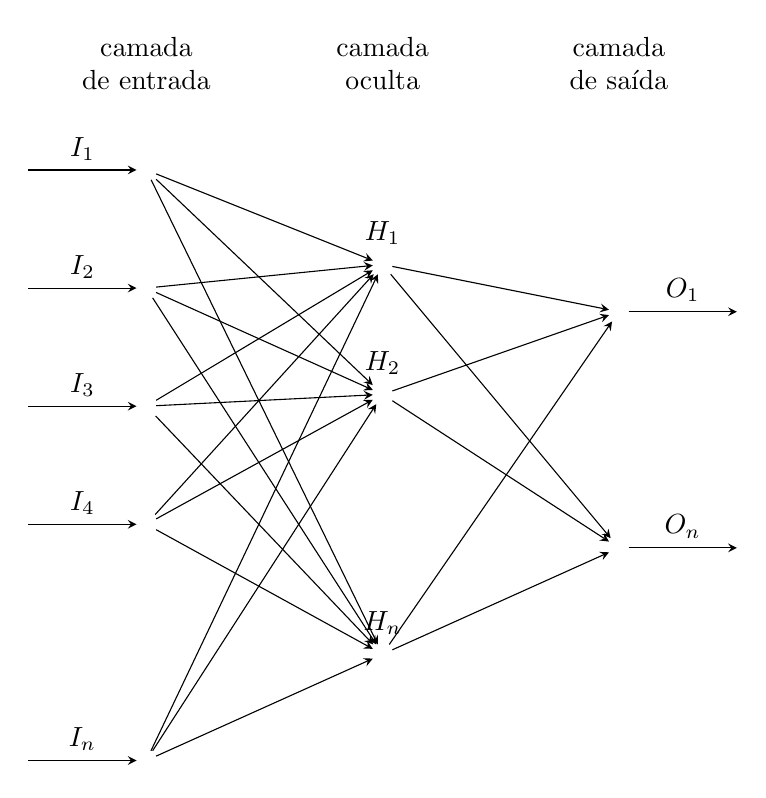
\begin{tikzpicture}[x=1.5cm, y=1.5cm, >=stealth]

\foreach \m/\l [count=\y] in {1,2,3,4,missing,5}
  \node [every input/.try, input \m/.try] (input-\m) at (0,2.7-\y) {};

\foreach \m [count=\y] in {1,2,missing,3}
  \node [every neuron/.try, neuron \m/.try ] (hidden-\m) at (2,2-\y*1.1) {};

\foreach \m [count=\y] in {1,missing,2}
  \node [every neuron/.try, neuron \m/.try ] (output-\m) at (4,1.5-\y) {};

\foreach \l [count=\i] in {1,2,3,4,n}
  \draw [<-] (input-\i) -- ++(-1,0)
    node [above, midway] {$I_\l$};

\foreach \l [count=\i] in {1,2,n}
  \node [above] at (hidden-\i.north) {$H_\l$};

\foreach \l [count=\i] in {1,n}
  \draw [->] (output-\i) -- ++(1,0)
    node [above, midway] {$O_\l$};

\foreach \i in {1,...,5}
  \foreach \j in {1,...,3}
    \draw [->] (input-\i) -- (hidden-\j);

\foreach \i in {1,...,3}
  \foreach \j in {1,...,2}
    \draw [->] (hidden-\i) -- (output-\j);

\foreach \l [count=\x from 0] in {de entrada, oculta, de sa\'ida}
  \node [align=center, above] at (\x*2,2.3) {camada \\ \l};

\end{tikzpicture}
            %%\begin{tikzpicture}[&gt;=stealth']
\begin{tikzpicture}
% Draw axes
%\draw [&lt;-&gt;,thick] (0,5) node (yaxis) [above] {$y$}
\draw [thick] (0,5) node (yaxis) [above] {$y$}
|- (5,0) node (xaxis) [right] {$x$};
% draw line
\draw (0,-1) -- (5,4); % y=x-1
\draw[dashed] (-1,0) -- (4,5); % y=x+1
\draw[dashed] (2,-1) -- (6,3); % y=x-3
\draw[black,<->,very thick]     (1.5,2.5)-- (3.5,0.5) node[above, rotate=-45,midway,xshift=-5]{$D$};% y=-x+4
% \draw labels
\draw (3.5,3) node[rotate=45,font=\small] 
{$\mathbf{w}\cdot \mathbf{x} + b = 0$};
\draw (2.5,4) node[rotate=45,font=\small] 
{$\mathbf{w}\cdot \mathbf{x} + b = 1$};
\draw (4.5,2) node[rotate=45,font=\small] 
{$\mathbf{w}\cdot \mathbf{x} + b = -1$};
% draw distance
%\draw[dotted] (4,5) -- (6,3);
%\draw (5.25,4.25) node[rotate=-45] {$\frac{2}{\Vert \mathbf{w} \Vert}$};
%\draw[dotted] (0,0) -- (0.5,-0.5);
%\draw (0,-0.5) node[rotate=-45] {$\frac{b}{\Vert \mathbf{w} \Vert}$};
%\draw[-&gt;] (2,1) -- (1.5,1.5);
%\draw[thick] (2,1) -- (1.5,1.5);
\draw (1.85,1.35) node[rotate=-45]{}; %{$\mathbf{w}$};
% draw negative dots
\fill[red] (0.5,1.5) circle (3pt);
\fill[red]   (2.5,3.5)   circle (3pt);
\fill[black] (1,2.5)     circle (3pt);
\fill[black] (0.75,2)    circle (3pt);
\fill[black] (0.6,1.9)   circle (3pt);
\fill[black] (0.77, 2.5) circle (3pt);
\fill[black] (1.5,3)     circle (3pt);
\fill[black] (1.3,3.3)   circle (3pt);
\fill[black] (0.6,3.2)   circle (3pt);
% draw positive dots
\draw[red,thick] (4,1)     circle (3pt); 
\draw[red,thick] (3.3,.3)  circle (3pt); 
\draw[black]     (4.5,1.2) circle (3pt); 
\draw[black]     (4.5,.5)  circle (3pt); 
\draw[black]     (3.9,.7)  circle (3pt); 
\draw[black]     (5,1)     circle (3pt); 
\draw[black]     (3.5,.2)  circle (3pt); 
\draw[black]     (4,.3)    circle (3pt); 
\end{tikzpicture}
            
            %\input{./graficos/KNN2.tex}
            }
            \end{column}
            \begin{column}{0.5\textwidth}
                \begin{itemize}
                    \item Camadas Ocultas com 20 Neuronios
                \end{itemize}
            \end{column}
    \end{columns}        
\end{frame}
%--------------------------------------------------

\begin{frame}{SVM}
    \begin{columns}
        \begin{column}{0.5\textwidth}            
            \color{black}
            
            %\scalebox{.4}{\tikzset{%
  every neuron/.style={
    circle,
    draw,
    minimum size=1cm
  },
  neuron missing/.style={
    draw=none, 
    scale=2,
    text height=0.333cm,
    execute at begin node=\color{black}$\vdots$
  },
  every input/.style={
  	rectangle,
  	draw,
  	minimum size=0.2cm
  },
  input missing/.style={
	draw=none, 
	scale=2,
	text height=0.333cm,
	execute at begin node=\color{black}$\vdots$
},
}

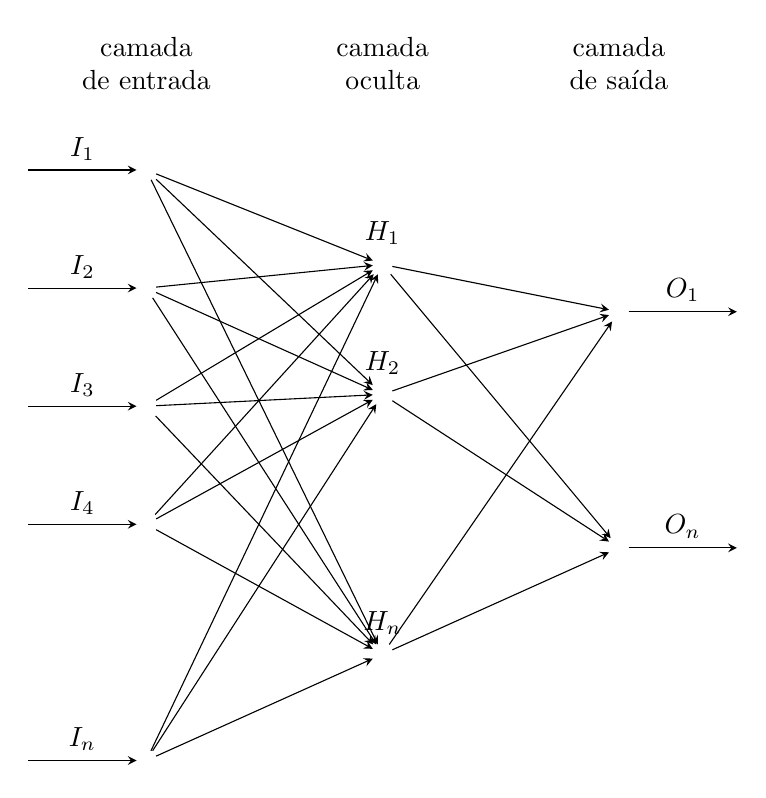
\begin{tikzpicture}[x=1.5cm, y=1.5cm, >=stealth]

\foreach \m/\l [count=\y] in {1,2,3,4,missing,5}
  \node [every input/.try, input \m/.try] (input-\m) at (0,2.7-\y) {};

\foreach \m [count=\y] in {1,2,missing,3}
  \node [every neuron/.try, neuron \m/.try ] (hidden-\m) at (2,2-\y*1.1) {};

\foreach \m [count=\y] in {1,missing,2}
  \node [every neuron/.try, neuron \m/.try ] (output-\m) at (4,1.5-\y) {};

\foreach \l [count=\i] in {1,2,3,4,n}
  \draw [<-] (input-\i) -- ++(-1,0)
    node [above, midway] {$I_\l$};

\foreach \l [count=\i] in {1,2,n}
  \node [above] at (hidden-\i.north) {$H_\l$};

\foreach \l [count=\i] in {1,n}
  \draw [->] (output-\i) -- ++(1,0)
    node [above, midway] {$O_\l$};

\foreach \i in {1,...,5}
  \foreach \j in {1,...,3}
    \draw [->] (input-\i) -- (hidden-\j);

\foreach \i in {1,...,3}
  \foreach \j in {1,...,2}
    \draw [->] (hidden-\i) -- (output-\j);

\foreach \l [count=\x from 0] in {de entrada, oculta, de sa\'ida}
  \node [align=center, above] at (\x*2,2.3) {camada \\ \l};

\end{tikzpicture}}
            %\scalebox{.5}{%\begin{tikzpicture}[&gt;=stealth']
\begin{tikzpicture}
% Draw axes
%\draw [&lt;-&gt;,thick] (0,5) node (yaxis) [above] {$y$}
\draw [thick] (0,5) node (yaxis) [above] {$y$}
|- (5,0) node (xaxis) [right] {$x$};
% draw line
\draw (0,-1) -- (5,4); % y=x-1
\draw[dashed] (-1,0) -- (4,5); % y=x+1
\draw[dashed] (2,-1) -- (6,3); % y=x-3
\draw[black,<->,very thick]     (1.5,2.5)-- (3.5,0.5) node[above, rotate=-45,midway,xshift=-5]{$D$};% y=-x+4
% \draw labels
\draw (3.5,3) node[rotate=45,font=\small] 
{$\mathbf{w}\cdot \mathbf{x} + b = 0$};
\draw (2.5,4) node[rotate=45,font=\small] 
{$\mathbf{w}\cdot \mathbf{x} + b = 1$};
\draw (4.5,2) node[rotate=45,font=\small] 
{$\mathbf{w}\cdot \mathbf{x} + b = -1$};
% draw distance
%\draw[dotted] (4,5) -- (6,3);
%\draw (5.25,4.25) node[rotate=-45] {$\frac{2}{\Vert \mathbf{w} \Vert}$};
%\draw[dotted] (0,0) -- (0.5,-0.5);
%\draw (0,-0.5) node[rotate=-45] {$\frac{b}{\Vert \mathbf{w} \Vert}$};
%\draw[-&gt;] (2,1) -- (1.5,1.5);
%\draw[thick] (2,1) -- (1.5,1.5);
\draw (1.85,1.35) node[rotate=-45]{}; %{$\mathbf{w}$};
% draw negative dots
\fill[red] (0.5,1.5) circle (3pt);
\fill[red]   (2.5,3.5)   circle (3pt);
\fill[black] (1,2.5)     circle (3pt);
\fill[black] (0.75,2)    circle (3pt);
\fill[black] (0.6,1.9)   circle (3pt);
\fill[black] (0.77, 2.5) circle (3pt);
\fill[black] (1.5,3)     circle (3pt);
\fill[black] (1.3,3.3)   circle (3pt);
\fill[black] (0.6,3.2)   circle (3pt);
% draw positive dots
\draw[red,thick] (4,1)     circle (3pt); 
\draw[red,thick] (3.3,.3)  circle (3pt); 
\draw[black]     (4.5,1.2) circle (3pt); 
\draw[black]     (4.5,.5)  circle (3pt); 
\draw[black]     (3.9,.7)  circle (3pt); 
\draw[black]     (5,1)     circle (3pt); 
\draw[black]     (3.5,.2)  circle (3pt); 
\draw[black]     (4,.3)    circle (3pt); 
\end{tikzpicture}}
            \vspace{1cm}
            \scalebox{.6}{
            %\tikzset{%
  every neuron/.style={
    circle,
    draw,
    minimum size=1cm
  },
  neuron missing/.style={
    draw=none, 
    scale=2,
    text height=0.333cm,
    execute at begin node=\color{black}$\vdots$
  },
  every input/.style={
  	rectangle,
  	draw,
  	minimum size=0.2cm
  },
  input missing/.style={
	draw=none, 
	scale=2,
	text height=0.333cm,
	execute at begin node=\color{black}$\vdots$
},
}

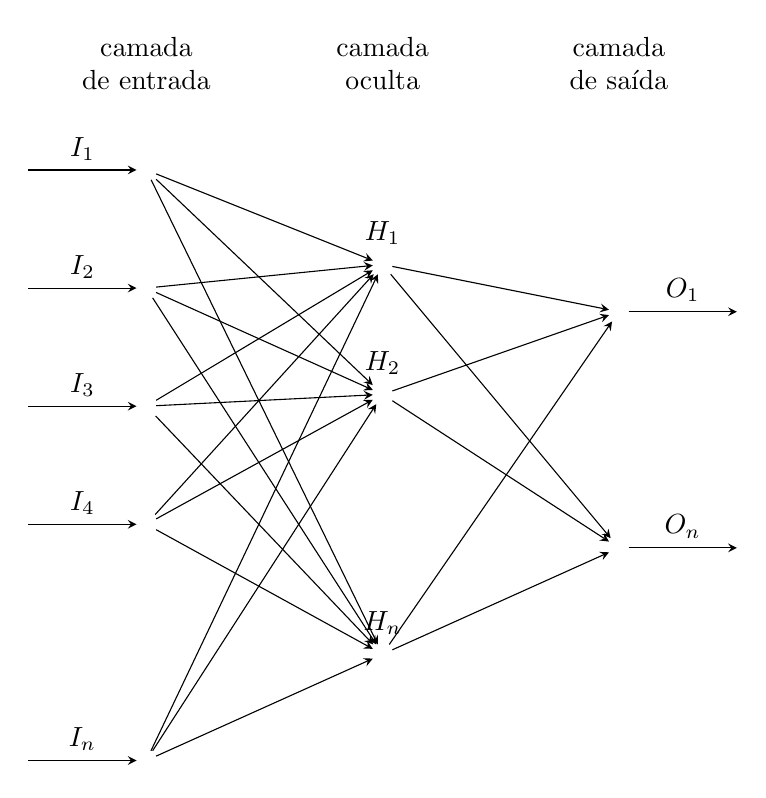
\begin{tikzpicture}[x=1.5cm, y=1.5cm, >=stealth]

\foreach \m/\l [count=\y] in {1,2,3,4,missing,5}
  \node [every input/.try, input \m/.try] (input-\m) at (0,2.7-\y) {};

\foreach \m [count=\y] in {1,2,missing,3}
  \node [every neuron/.try, neuron \m/.try ] (hidden-\m) at (2,2-\y*1.1) {};

\foreach \m [count=\y] in {1,missing,2}
  \node [every neuron/.try, neuron \m/.try ] (output-\m) at (4,1.5-\y) {};

\foreach \l [count=\i] in {1,2,3,4,n}
  \draw [<-] (input-\i) -- ++(-1,0)
    node [above, midway] {$I_\l$};

\foreach \l [count=\i] in {1,2,n}
  \node [above] at (hidden-\i.north) {$H_\l$};

\foreach \l [count=\i] in {1,n}
  \draw [->] (output-\i) -- ++(1,0)
    node [above, midway] {$O_\l$};

\foreach \i in {1,...,5}
  \foreach \j in {1,...,3}
    \draw [->] (input-\i) -- (hidden-\j);

\foreach \i in {1,...,3}
  \foreach \j in {1,...,2}
    \draw [->] (hidden-\i) -- (output-\j);

\foreach \l [count=\x from 0] in {de entrada, oculta, de sa\'ida}
  \node [align=center, above] at (\x*2,2.3) {camada \\ \l};

\end{tikzpicture}
            %\begin{tikzpicture}[&gt;=stealth']
\begin{tikzpicture}
% Draw axes
%\draw [&lt;-&gt;,thick] (0,5) node (yaxis) [above] {$y$}
\draw [thick] (0,5) node (yaxis) [above] {$y$}
|- (5,0) node (xaxis) [right] {$x$};
% draw line
\draw (0,-1) -- (5,4); % y=x-1
\draw[dashed] (-1,0) -- (4,5); % y=x+1
\draw[dashed] (2,-1) -- (6,3); % y=x-3
\draw[black,<->,very thick]     (1.5,2.5)-- (3.5,0.5) node[above, rotate=-45,midway,xshift=-5]{$D$};% y=-x+4
% \draw labels
\draw (3.5,3) node[rotate=45,font=\small] 
{$\mathbf{w}\cdot \mathbf{x} + b = 0$};
\draw (2.5,4) node[rotate=45,font=\small] 
{$\mathbf{w}\cdot \mathbf{x} + b = 1$};
\draw (4.5,2) node[rotate=45,font=\small] 
{$\mathbf{w}\cdot \mathbf{x} + b = -1$};
% draw distance
%\draw[dotted] (4,5) -- (6,3);
%\draw (5.25,4.25) node[rotate=-45] {$\frac{2}{\Vert \mathbf{w} \Vert}$};
%\draw[dotted] (0,0) -- (0.5,-0.5);
%\draw (0,-0.5) node[rotate=-45] {$\frac{b}{\Vert \mathbf{w} \Vert}$};
%\draw[-&gt;] (2,1) -- (1.5,1.5);
%\draw[thick] (2,1) -- (1.5,1.5);
\draw (1.85,1.35) node[rotate=-45]{}; %{$\mathbf{w}$};
% draw negative dots
\fill[red] (0.5,1.5) circle (3pt);
\fill[red]   (2.5,3.5)   circle (3pt);
\fill[black] (1,2.5)     circle (3pt);
\fill[black] (0.75,2)    circle (3pt);
\fill[black] (0.6,1.9)   circle (3pt);
\fill[black] (0.77, 2.5) circle (3pt);
\fill[black] (1.5,3)     circle (3pt);
\fill[black] (1.3,3.3)   circle (3pt);
\fill[black] (0.6,3.2)   circle (3pt);
% draw positive dots
\draw[red,thick] (4,1)     circle (3pt); 
\draw[red,thick] (3.3,.3)  circle (3pt); 
\draw[black]     (4.5,1.2) circle (3pt); 
\draw[black]     (4.5,.5)  circle (3pt); 
\draw[black]     (3.9,.7)  circle (3pt); 
\draw[black]     (5,1)     circle (3pt); 
\draw[black]     (3.5,.2)  circle (3pt); 
\draw[black]     (4,.3)    circle (3pt); 
\end{tikzpicture}
            
            %\input{./graficos/KNN2.tex}
            }
            \end{column}
            \begin{column}{0.5\textwidth}
                \begin{itemize}
                    \item Kernel Gaussian ("Fino", "Grosso")
                    \item Kernel Linear
                \end{itemize}
            \end{column}
    \end{columns}        
\end{frame}
%--------------------------------------------------

\begin{frame}{Compare Methods}
\begin{center}
\color{black}
\scalebox{.75}{
	\tikzstyle{block} = [
		% The shape:
		rectangle split,
		rectangle split parts =1,
		% The size:
		minimum size=6mm,
		draw,
		text badly centered,
		draw=blue!80!black!40,
		text=black,
	]
\tikzstyle{decision} = [
		diamond,
		draw,
		text badly centered,
		color=blue,
		aspect=2,
		inner sep=1.5pt,
		scale=0.7,
]
\tikzstyle{begin} = [
		rounded rectangle,
		draw,
		text badly centered,
		minimum size = 1cm,
		color=blue,
]
\tikzstyle{input} = [
ellipse,
draw,
text badly centered,
minimum size = 1cm,
color=blue,
]
\tikzstyle{coord} = [
-stealth,
inner sep =0 pt,
]
\begin{tikzpicture}[node distance= 0.6cm,
transition/.style={very thick,->}
]

\node [begin] (start) {\textbf{In\'icio itera\c{c}\~ao}};
\node[block,rectangle split parts=2] (Sujeito) [below=of start] {\nodepart{one}Sele\c{c}\~ao
	 \nodepart{two} Sujeito};
\node[block,rectangle split parts=2] (DB) [below=of Sujeito]{\nodepart{one}Obten\c{c}\~ao \nodepart{two} Database};
\node[block,rectangle split parts=2] (Dataset) [below=of DB] {\nodepart{one} Obten\c{c}\~ao
\nodepart{two} Dataset};
\node[block,rectangle split parts=1](Train) [below=of Dataset]{
	\nodepart{one} Treinamento classificador
};
\node[block,rectangle split parts=1] (Avaliacao1) [below=of Train]{Avalia\c{c}\~ao performance por Janela amostrada};
%\node []
\draw [transition] (start) -> (Sujeito);
\draw [transition] (Sujeito) -> (DB);
\draw [transition] (DB) -> (Dataset);
\draw [transition] (Dataset) -> (Train);
\draw [transition] (Train) -> (Avaliacao1);
\end{tikzpicture}}
\end{center}
\end{frame}


%--------------------------------------------------
\begin{frame}{Database}
\begin{center}
\color{black}
\scalebox{.95}{
	\tikzstyle{class} = [rectangle split,rectangle split parts=1,draw ,text badly centered, node distance=1cm,scale=0.9]
\begin{tikzpicture}
[edge from parent fork down,sibling distance=4cm,level distance=7cm,
edge from parent/.style={draw,<-,line width=1.2pt}]
\node[class,rectangle split parts=2](Database)
	{
	\nodepart{one}  \textcolor{blue}{\large{Database}}
	 \nodepart{two} \begin{tabular}{cc}
					\textcolor{purple}{Database}(overlap,windowLength,Trials)\\
					\textcolor{purple}{getSampleCountPerLabel}()\\
					\textcolor{purple}{generateDatasetIndex}(numSamples)\\
					\textcolor{purple}{generateDataset}(TrainingDataset)\\
					\textcolor{purple}{getSample}(Range)\\
					\textcolor{purple}{getSampleCount}()\\
					\textcolor{purple}{setFeatureExtractionFcn}(FEFunction)\\
					\end{tabular}
				
};
\end{tikzpicture}}
\end{center}
\end{frame}
%--------------------------------------------------
\begin{frame}{Feature Extraction}
\begin{center}
\color{black}
\scalebox{.8}{
	\tikzstyle{class} = [rectangle split,rectangle split parts=1,draw ,text badly centered, node distance=1cm,scale=0.7]
\begin{tikzpicture}
[edge from parent fork down,sibling distance=5cm,level distance=4cm,
edge from parent/.style={draw,<-,line width=1.2pt}]
\node[class,rectangle split parts=2](FeatureExtractionFnc)
	{
	\nodepart{one}  \textcolor{blue}{\large{\textit{FeatureExtractionFnc}}}
	 \nodepart{two} \begin{tabular}{cc}
	 					 \textit{\textcolor{purple}{ExtractFeature}}(C3,Cz,C4)\\
					\end{tabular}
	}
	child{ node [class, rectangle split parts=2] (PWelch)
		{
		\nodepart{one} \large{\textcolor{blue}{PWelch}}
		\nodepart{two} \begin{tabular}{cc}
							\textcolor{purple}{ExtractFeature}(C3,Cz,C4)\\
						\end{tabular}
		}
	}
	child{ node [class, rectangle split parts=2] (PSD)
		{
		\nodepart{one} \large{\textcolor{blue}{PSD}}
		\nodepart{two} \begin{tabular}{cc}
		\textcolor{purple}{ExtractFeatures}(C3,Cz,C4)\\
		\end{tabular}
		}
	}
	child{ node [class, rectangle split parts=2] (PMTM)
		{
		\nodepart{one} \large{\textcolor{blue}{PMTM}}
		\nodepart{two} \begin{tabular}{cc}
		\textcolor{purple}{ExtractFeatures}(C3,Cz,C4)\\
		\end{tabular}
		}
	};
\end{tikzpicture}}
\end{center}
\end{frame}
%--------------------------------------------------
\begin{frame}{Classifier}
\begin{center}
\color{black}
\scalebox{.75}{
	\tikzstyle{class} = [rectangle split,rectangle split parts=1,draw ,text badly centered, node distance=1cm,scale=0.7]
\begin{tikzpicture}
[edge from parent fork down,sibling distance=4cm,level distance=7cm,
edge from parent/.style={draw,<-,line width=1.2pt}]
\node[class,rectangle split parts=3](Classifier)
	{
	\nodepart{one}  \textcolor{blue}{\large{\textit{Classifier}}}
	 \nodepart{two} \begin{tabular}{cc}
	 					 \textit{\textcolor{purple}{train}}()\\
 						 \textit{\textcolor{purple}{predict}}()\\
					\end{tabular}
	 \nodepart{three} \begin{tabular}{cc}
					\textcolor{purple}{calculatePerformance}(ValidationSet)\\
					\textcolor{purple}{exportModel}()\\
					\textcolor{purple}{loadModel}(Model)\\
					\textcolor{purple}{loadTrainingData}(TrainingDataset)\\
					\end{tabular}
				
	}
	child{ node [class, rectangle split parts=2] (LinearSVM)
		{
		\nodepart{one} \large{\textcolor{blue}{LinearSVM}}
		\nodepart{two} \begin{tabular}{cc}
							\textcolor{purple}{LinearSVM}()\\
							\textcolor{purple}{train}()\\
							\textcolor{purple}{predict}()\\
						\end{tabular}
		}
	}
	child{ node [class, rectangle split parts=2] (gaussianSVM)
		{
		\nodepart{one} \large{\textcolor{blue}{gaussianSVM}}
		\nodepart{two} \begin{tabular}{cc}
		\textcolor{purple}{gaussianSVM}(KernelScale)\\
		\textcolor{purple}{train}()\\
		\textcolor{purple}{predict}()\\
		\end{tabular}
		}
	}
	child{ node [class, rectangle split parts=2] (kNN)
		{
		\nodepart{one} \large{\textcolor{blue}{kNN}}
		\nodepart{two} \begin{tabular}{cc}
		\textcolor{purple}{kNN}(numNeighbours)\\
		\textcolor{purple}{train}()\\
		\textcolor{purple}{predict}()\\
		\end{tabular}
		}
	}
	child{ node [class, rectangle split parts=2] (ANN)
		{
			\nodepart{one} \large{\textcolor{blue}{ANN}}
			\nodepart{two} \begin{tabular}{cc}
			\textcolor{purple}{ANN}(Layers)\\
			\textcolor{purple}{train}()\\
			\textcolor{purple}{predict}()\\
			\end{tabular}
		}
};
\end{tikzpicture}}
\end{center}
\end{frame}

%----------------------------------------------------------------------------------------
%	 Resultados
%----------------------------------------------------------------------------------------

%\section{Resultados}


\begin{frame}{Overlap e Janelas de Amostragem}
\color{black}
    \scalebox{.6}{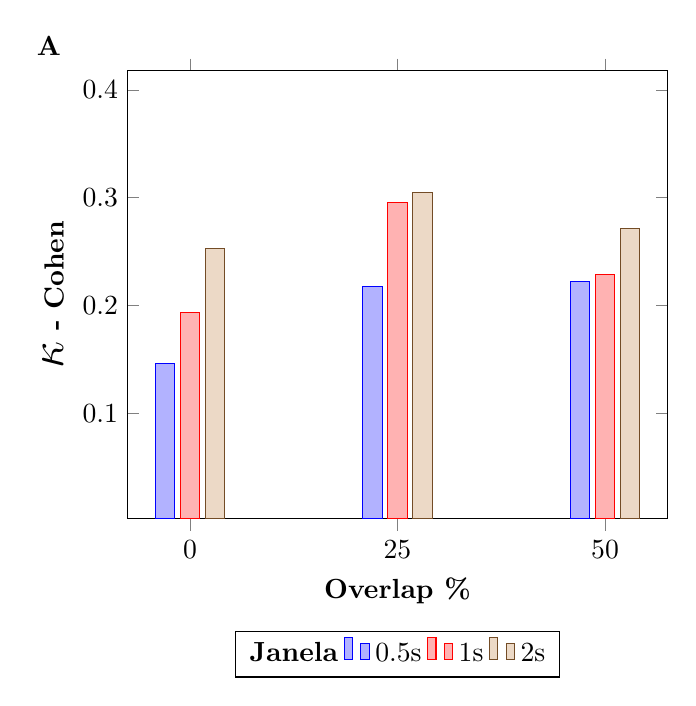
\begin{tikzpicture}
\begin{axis}[ybar,
ylabel={\textbf{{\LARGE $\kappa$} - Cohen}},
symbolic x coords={0,25,50},
enlargelimits=0.15,
bar width=7pt,
xlabel=\textbf{{Overlap \%}},
scale=1,
ymin=0.05,
ymax=0.37,
xtick=data,
legend style={at={(0.5,-0.25)},anchor=north,legend columns=-1},
]
\addlegendimage{empty legend}
\addlegendentry[]{\textbf{Janela}  }


\addplot coordinates{
	(0,0.145756921970514)
	(25,0.217953198653199)
	(50,0.222418529316488)
	
};
\addlegendentry{0.5s}
\addplot coordinates {
	(0,0.193445731381201)
	(25,0.295532180595581)
	(50,0.228335707502374)
};
\addlegendentry{1s}
\addplot coordinates {
	(0,0.253022486772487)
	(25,0.305006613756614)
	(50,0.271798941798942)
};
\addlegendentry{2s}

\end{axis}
\node[] at (-1,6) {\textbf{A}};
\end{tikzpicture}}
    \scalebox{.6}{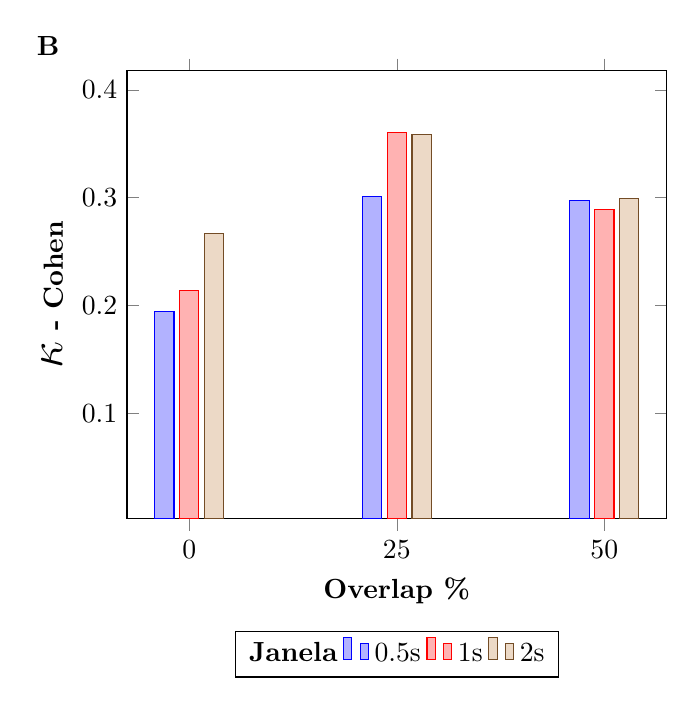
\begin{tikzpicture}
\begin{axis}[ybar,
ylabel={\textbf{{\LARGE $\kappa$} - Cohen}},
symbolic x coords={0,25,50},
enlargelimits=0.15,
bar width=7pt,
xlabel=\textbf{{Overlap \%}},
scale=1,
ymin=0.05,
ymax=0.37,
xtick=data,
legend style={at={(0.5,-0.25)},anchor=north,legend columns=-1},
]

\addlegendimage{empty legend}
\addlegendentry[]{\textbf{Janela}  }

\addplot coordinates{
	(0,0.194592780487009)
	(25,0.301151008868141)
	(50,0.297452810791095)
	
};
\addlegendentry{0.5s}
\addplot coordinates {
	(0,0.213851347718643)
	(25,0.360070705941324)
	(50,0.288910829755114)
};
\addlegendentry{1s}
\addplot coordinates {
	(0,0.2669239009365)
	(25,0.358554160497779)
	(50,0.299020891771033)
};
\addlegendentry{2s}
\end{axis}
\node[] at (-1,6) {\textbf{B}};
\end{tikzpicture}}
\end{frame}
\begin{frame}{Classificadores e Extração de Caracteristicas}
\color{black}
    \scalebox{.5}{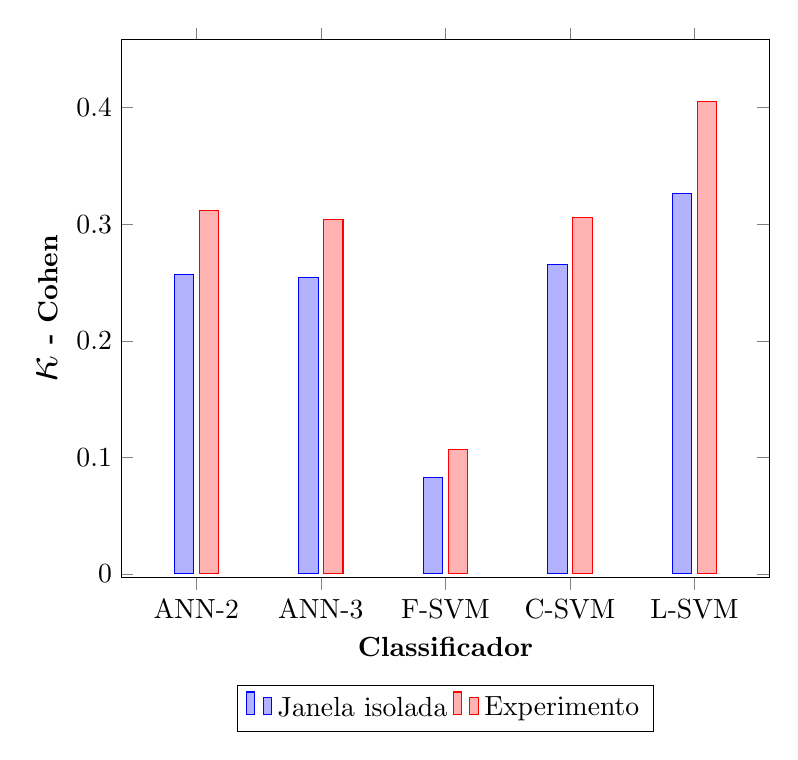
\begin{tikzpicture}
\begin{axis}[ybar,
ylabel={\textbf{{\LARGE $\kappa$} - Cohen}},
symbolic x coords={ANN-2,ANN-3,F-SVM,C-SVM,L-SVM},
enlargelimits=0.15,
bar width=7pt,
xlabel={\textbf{Classificador}},
xtick=data,
legend style={at={(0.5,-0.2)},anchor=north,legend columns=-1},
scale=1.2,
ymin=0.05,
]
\addplot coordinates {
	(ANN-2,0.256710322461084)
	(ANN-3,0.253969286000733)
	(F-SVM,0.08251886405747)
	(C-SVM,0.265203892414323)
	(L-SVM,0.32674780825939)
};
\addplot coordinates {
	(ANN-2,0.311612621296827)
	(ANN-3,0.304360005958168)
	(F-SVM,0.106615596193986)
	(C-SVM,0.305949166653495)
	(L-SVM,0.405089519212324)
};
\legend{Janela isolada,Experimento}
\end{axis}
\end{tikzpicture}}
    \scalebox{.5}{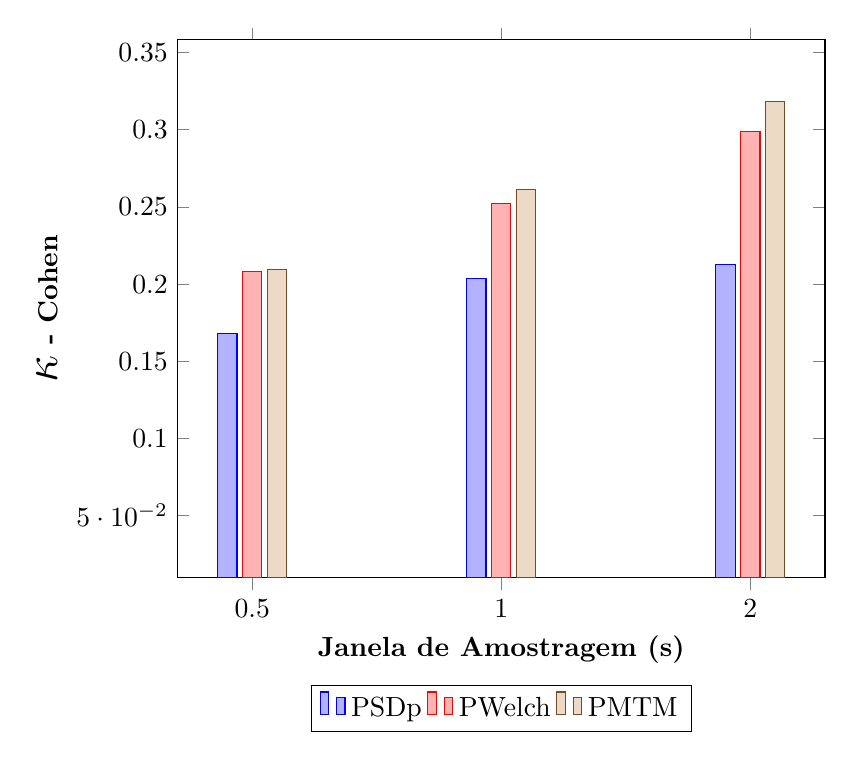
\begin{tikzpicture}
\begin{axis}[ybar,
ylabel={\textbf{{\LARGE $\kappa$} - Cohen}},
symbolic x coords={0.5,1,2},
enlargelimits=0.15,
bar width=7pt,
xlabel={\textbf{Janela de Amostragem (s)}},
xtick=data,
legend style={at={(0.5,-0.2)},anchor=north,legend columns=-1},
scale=1.2,
ymin=0.05,
]

\addplot coordinates {

	(0.5,0.168200019315786)
	(1,0.20381375312512)
	(2,0.212802028218695)

};
\addlegendentry[]{PSDp}
\addplot coordinates {
	(0.5,0.208379846569074)
	(1,0.252435974315611)
	(2,0.298970458553792)
};
\addlegendentry[]{PWelch}
\addplot coordinates {
	(0.5,0.209548784055341)
	(1,0.261063892038425)
	(2,0.318055555555556)
};
\addlegendentry[]{PMTM}
\end{axis}
\end{tikzpicture}}
\end{frame}


%------------------------------------------------------------------------
\begin{frame}{Melhores Performances}
\color{black}
 \centering% used instead the environment center
    \begin{table}[h!]
	\caption{Melhores performances na m\'etrica do experimento}
	\scriptsize
	\begin{tabularx}{\textwidth}{c|c|c|c|c|c|c|c|c}
		\hline\hline
		Pos&$\kappa_1$ &$\text{ACC}_1$&$\kappa_2$&$\text{ACC}_2$&Janela& Overlap&Fun\c{c}\~ao&Classificador  \\ \hline 
		$1^{\underline{o}}$&0.422&71.14\%&0.526&76.32\%&2s&25\%&PWelch&\acs{L-SVM} \\ \hline 
		$2^{\underline{o}}$&0.426&71.35\%&0.512&75.62\%&2s&25\%&PMTM&L-SVM \\ \hline
		$3^{\underline{o}}$&0.421&71.06\%&0.491&74.58\%&2s&25\%&PMTM&\acs{ANN-3} \\ \hline
		$4^{\underline{o}}$&0.407&70.36\%&0.490&74.51\%&1s&25\%&PMTM&L-SVM \\ \hline
		$5^{\underline{o}}$&0.402&70.11\%&0.484&74.23\%&1s&25\%&PMTM&\ac{ANN-2} \\ \hline
	\end{tabularx}
	
	\label{Tab:melhoresKappaFull}
\end{table}
\end{frame}
%------------------------------------------------------------------------
\begin{frame}{Melhores Performances}
\color{black}
\centering

\begin{table}[h!]

	\caption{Melhores performances por Janela de amostragem de at\'e 2s}
	\scriptsize
	\begin{tabularx}{\textwidth}{c|c|c|c|c|c|c|c|c}		
		\hline\hline
		Pos&$\kappa_1$ &$\text{ACC}_1$&$\kappa_2$&$\text{ACC}_2$&Janela& Overlap&Fun\c{c}\~ao&Classificador  \\ \hline
		$1^{\underline{o}}$&0.426&71.35\%&0.512&75.62\%&2s&25\%&PMTM&L-SVM \\ \hline 
		$2^{\underline{o}}$&0.422&71.14\%&0.526&76.32\%&2s&25\%&PWelch&L-SVM\\ \hline
		$3^{\underline{o}}$&0.421&71.07\%&0.452&72.61\%&2s&0\%&PMTM&L-SVM \\ \hline
		$4^{\underline{o}}$&0.421&71.06\%&0.491&74.58\%&2s&25\%&PMTM&ANN-3 \\ \hline
		$5^{\underline{o}}$&0.418&70.95\%&0.466&73.33\%&2s&50\%&PMTM&L-SVM \\ \hline
	\end{tabularx}
	\label{Tab:melhoresKappa}

\end{table}

\end{frame}

%------------------------------------------------------------------------

\begin{frame}{Melhores Performances}
\color{black}
\centering

\begin{table}[h!]
	\caption{Melhores performances por Janela de amostragem de at\'e 0.5s}
	\scriptsize
	\begin{tabularx}{\textwidth}{c|c|c|c|c|c|c|c|c}		
		\hline\hline
		Pos&$\kappa_1$ &$\text{ACC}_1$&$\kappa_2$&$\text{ACC}_2$&Janela& Overlap&Fun\c{c}\~ao&Classificador  \\ \hline
		$1^{\underline{o}}$&0.293&64.69\%&0.401&70.09\%&0.5s&	50\%&PMTM&L-SVM \\ \hline 
		$2^{\underline{o}}$&0.286&64.31\%&0.388&69.45\%&0.5s&	50\%&PWelch&L-SVM \\ \hline
		$3^{\underline{o}}$&0.284&64,21\%&0.399&69.98\%&0.5s&25\%&PMTM&L-SVM \\ \hline
		$4^{\underline{o}}$&0.280&64,01\%&0.397&69.88\%&0.5s&25\%&PWelch&L-SVM \\ \hline
		$5^{\underline{o}}$&0.275&63.78\%&0.391&69.57\%&0.5s&	25\%&PMTM&ANN-2 \\ \hline
	\end{tabularx}
	\label{Tab:melhoresKappa125}
\end{table}

\end{frame}



%----------------------------------------------------------------------------------------
%	 Conclusoes
%----------------------------------------------------------------------------------------


%\section{Conclusões}
\begin{frame}{Conclus\~ao}
\color{BLACK}%ER
\begin{table}[h!]
	\centering
	\tiny
	\caption{Resultados da competi\c{c}\~ao BCI-IV 2008}
	\begin{tabularx}{\textwidth}{c|X|c|c|c|c|c|c|c|c|c|c}		
		\hline\hline
		Pos&contributor&$\kappa$&1&2&3&4&5&6&7&8&9  \\ \hline
		$1^{\underline{o}}$&Z. Y. Chin&\textbf{0.60}&0.40&0.21&0.22&	0.95&0.86&0.61&0.56&0.85&0.74 \\ \hline 
		$2^{\underline{o}}$&H. Gan&\textbf{0.58}&0.42&0.21&0.14&0.94&0.71 &0.62&0.61&0.84&0.78 \\ \hline
		$3^{\underline{o}}$&D. Coyle&\textbf{0.46}&0.19&0.12&0.12 &0.77&0.57&0.49&0.38&0.85&0.61 \\ \hline
		$4^{\underline{o}}$&S. Lodder&\textbf{0.43}&0.23&0.31&0.07&0.91& 	0.24&0.42&0.41&0.74&0.53 \\ \hline
		$5^{\underline{o}}$&J. F. D. Saa&\textbf{0.37}&0.20&0.16&0.16&0.73&0.21&0.19&0.39&0.86&0.44 \\ \hline
		$6^{\underline{o}}$&Y. Ping&\textbf{0.25}&0.02&0.09&0.07&0.43&0.25&0.00&0.14&0.76&0.47\\ \hline\hline
		-&L-SVM PMTM&\textbf{0.51}&0.41&0&0.09&0.92&0.58&0.63&0.4&0.83&0.71\\ \hline
	\end{tabularx}
	\label{Tab:BCI2008}
\end{table}
\end{frame}



\iffalse
%------------------------------------------------

\begin{frame}[plain]{Plain Slide}
	This is a slide with the plain style and it is numbered.
\end{frame}

%------------------------------------------------

\begin{frame}[t]
	This slide has an empty title and is aligned to top.
\end{frame}

%------------------------------------------------

\begin{frame}[noframenumbering]{No Slide Numbering}
	This slide is not numbered and is citing reference \cite{knuth74}.
\end{frame}

%------------------------------------------------

\begin{frame}{Typesetting and Math}
	The packages \texttt{inputenc} and \texttt{FiraSans}\footnote{\url{https://fonts.google.com/specimen/Fira+Sans}}\textsuperscript{,}\footnote{\url{http://mozilla.github.io/Fira/}} are used to properly set the main fonts.
	\vfill
	This theme provides styling commands to typeset \emph{emphasized}, \alert{alerted}, \textbf{bold}, \textcolor{example}{example text}, \dots
	\vfill
	\texttt{FiraSans} also provides support for mathematical symbols:
	\begin{equation*}
		e^{i\pi} + 1 = 0.
	\end{equation*}
\end{frame}



%----------------------------------------------------------------------------------------
%	 SECTION 2
%----------------------------------------------------------------------------------------

%------------------------------------------------
%%%
\begin{frame}{Blocks}
	These blocks are part of 1 slide, to be displayed consecutively.
	\begin{block}{Block}
		Text.
	\end{block}
	\pause % Automatically creates a new "page" split between the above and above + below
	\begin{alertblock}{Alert block}
		Alert \alert{text}.
	\end{alertblock}
	\pause % Automatically creates a new "page" split between the above and above + below
	\begin{exampleblock}{Example block}
		Example \textcolor{example}{text}.
	\end{exampleblock}
\end{frame}

%------------------------------------------------

\begin{frame}{Columns}
	\begin{columns}
		\column{0.5\textwidth}
			This text appears in the left column and wraps neatly with a margin between columns.
		
		\column{0.5\textwidth}
			
\includegraphics[width=\linewidth]{Images/placeholder.jpg}
	\end{columns}
\end{frame}

%------------------------------------------------

\begin{frame}{Lists}
	\begin{columns}[T, onlytextwidth] % T for top align, onlytextwidth to suppress the margin between columns
		\column{0.33\textwidth}
			Items:
			\begin{itemize}
				\item Item 1
				\begin{itemize}
					\item Subitem 1.1
					\item Subitem 1.2
				\end{itemize}
				\item Item 2
				\item Item 3
			\end{itemize}
		
		\column{0.33\textwidth}
			Enumerations:
			\begin{enumerate}
				\item First
				\item Second
				\begin{enumerate}
					\item Sub-first
					\item Sub-second
				\end{enumerate}
				\item Third
			\end{enumerate}
		
		\column{0.33\textwidth}
			Descriptions:
			\begin{description}
				\item[First] Yes.
				\item[Second] No.
			\end{description}
	\end{columns}
\end{frame}

%------------------------------------------------

\begin{frame}{Table}
	\begin{table}
		\centering % Centre the table on the slide
		\begin{tabular}{l c}
			\toprule
			Discipline & Avg. Salary \\
			\toprule
			\textbf{Engineering} & \textbf{\$66,521} \\
			Computer Sciences & \$60,005\\
			Mathematics and Sciences & \$61,867\\
			Business & \$56,720\\
			Humanities \& Social Sciences & \$56,669\\
			Agriculture and Natural Resources & \$53,565\\
			Communications & \$51,448\\
			\midrule
			\textbf{Average for All Disciplines} & \textbf{\$58,114}\\
			\bottomrule
		\end{tabular}
	\caption{Table caption}
	\end{table}
\end{frame}
\begin{frame}{Conclus\~ao}
\color{BLACK}%ER
\tiny
\begin{table}[h!]
	\centering
	\caption{Resultados da competi\c{c}\~ao BCI-IV 2008}
	\begin{tabularx}{\textwidth}{c|X|c|c|c|c|c|c|c|c|c|c}		
		\hline\hline
		Pos&contributor&$\kappa$&1&2&3&4&5&6&7&8&9  \\ \hline
		$1^{\underline{o}}$&Z. Y. Chin&\textbf{0.60}&0.40&0.21&0.22&	0.95&0.86&0.61&0.56&0.85&0.74 \\ \hline 
		$2^{\underline{o}}$&H. Gan&\textbf{0.58}&0.42&0.21&0.14&0.94&0.71 &0.62&0.61&0.84&0.78 \\ \hline
		$3^{\underline{o}}$&D. Coyle&\textbf{0.46}&0.19&0.12&0.12 &0.77&0.57&0.49&0.38&0.85&0.61 \\ \hline
		$4^{\underline{o}}$&S. Lodder&\textbf{0.43}&0.23&0.31&0.07&0.91& 	0.24&0.42&0.41&0.74&0.53 \\ \hline
		$5^{\underline{o}}$&J. F. D. Saa&\textbf{0.37}&0.20&0.16&0.16&0.73&0.21&0.19&0.39&0.86&0.44 \\ \hline
		$6^{\underline{o}}$&Y. Ping&\textbf{0.25}&0.02&0.09&0.07&0.43&0.25&0.00&0.14&0.76&0.47\\ \hline\hline
		-&L-SVM PMTM&\textbf{0.51}&0.41&0&0.09&0.92&0.58&0.63&0.4&0.83&0.71\\ \hline
	\end{tabularx}
	\label{Tab:BCI2008}
\end{table}
\end{frame}
%------------------------------------------------
\begin{frame}{Trabalhos Futuros}

CNN
\end{frame}


\begin{frame}[focus]
	Thanks for using \textbf{Focus}!
\end{frame}
\fi

%----------------------------------------------------------------------------------------
%	 CLOSING/SUPPLEMENTARY SLIDES
%----------------------------------------------------------------------------------------

\appendix

\begin{frame}{Referencias}
	%\nocite{*} % Display all references regardless of if they were cited

	\bibliography{bibliografia.bib}
	\bibliographystyle{plain}
\end{frame}

%------------------------------------------------

\begin{frame}[focus]
AGRADECIMENTOS
\vfill
%PQ DEUS NOS ABANDONOU ? 
%PQ?

\end{frame}

%----------------------------------------------------------------------------------------

\end{document}
